\documentclass[11pt,a4paper]{article}

% ============================================================================
% PACKAGES
% ============================================================================
\usepackage[utf8]{inputenc}
\usepackage[T1]{fontenc}
\usepackage{amsmath,amssymb,amsthm}
\usepackage{graphicx}
\usepackage{booktabs}
\usepackage{siunitx}
\usepackage{algorithm}
\usepackage{algpseudocode}
\usepackage[hyphens]{url}
\usepackage[colorlinks=true,citecolor=blue,linkcolor=blue,urlcolor=blue]{hyperref}
\usepackage[backend=biber,style=numeric,sorting=none]{biblatex}
\usepackage{caption}
\usepackage{subcaption}
\usepackage{multirow}
\usepackage{array}
\usepackage{xcolor}

% Keep the editing wrapper available without revision-color markup.
\newcommand{\rev}[1]{#1}

% ============================================================================
% BIBLIOGRAPHY
% ============================================================================
\addbibresource{references.bib}

% ============================================================================
% FORMATTING
% ============================================================================
\setlength{\parindent}{0pt}
\setlength{\parskip}{6pt}

\captionsetup{font=small,labelfont=bf}

% ============================================================================
% METADATA
% ============================================================================
\title{\textbf{Shape-First Electricity Load Segmentation: Controlled Synthetic Validation and Unsupervised Analysis of Real Client Data}}

\author{
  Shantanu\\[6pt]
  \small ORCID: \href{https://orcid.org/0009-0008-4403-0670}{0009-0008-4403-0670}\\
  \small Thapar Institute of Engineering and Technology\\
  \small Department of Electronics and Communication Engineering\\
  \small \texttt{sshantanu\_be25@thapar.edu}
}

\date{}

% ============================================================================
% DOCUMENT
% ============================================================================
\begin{document}

\maketitle

% ============================================================================
% ABSTRACT
% ============================================================================
\begin{abstract}
We evaluate a reproducible shape-first electricity-load clustering pipeline in two settings. In a controlled synthetic experiment with 200 consumers over 365 days, the selected four-cluster solution attains an Adjusted Rand Index (ARI) of 0.813 against hidden archetype labels. Across 20 shorter synthetic datasets, magnitude-only features have near-zero mean archetype recovery (ARI 0.013), despite a higher silhouette than the behavioral representation. In a separate unsupervised analysis of the UCI ElectricityLoadDiagrams20112014 dataset, a seeded sample of 120 client columns for 2012 contained 16 all-zero clients, which were excluded because normalized load shapes are undefined for them; the remaining 104 clients produced 913,536 hourly records. The pipeline selected K=2, the only candidate from K=2--8 to meet its five-percent minimum cluster-size rule. Eight K-means restarts yielded pairwise ARI 1.000, while independently fitted partitions across three chronological windows had mean pairwise ARI 0.288. These measured-data results show a reproducible full-year fit but weak persistence across time windows; they do not establish behavioral ground truth or household-specific patterns. The UCI clients are not assumed to be households. We report the synthetic and measured-data analyses separately and provide the source hash, sampling record, script, and outputs for replication.

\textbf{Keywords:} electricity load profiles, client segmentation, shape normalization, PCA, K-means, unsupervised validation, reproducible research, smart meter analytics
\end{abstract}

% ============================================================================
% 1. INTRODUCTION
% ============================================================================
\section{Introduction}
\label{sec:introduction}

The widespread deployment of smart meters has enabled high-resolution monitoring of household electricity consumption at unprecedented scale \cite{lazar2021investigating,kwac2014household}. This granular data enables segmentation of consumers into behaviorally distinct groups, supporting targeted demand response programs, dynamic pricing strategies, and infrastructure planning \cite{yan2021multiple,abdullah2025ml}. However, traditional clustering approaches often group households primarily by total consumption magnitude---how much energy they use---rather than by temporal usage patterns---when energy is consumed \cite{jin2016loadshape,rhodes2014clustering}.

Magnitude-based segmentation conflates two independent dimensions: a household's energy intensity (driven by building size, occupancy, appliances) and its behavioral routine (driven by occupancy patterns, work schedules, lifestyle preferences). Two households with identical daily load shapes but different consumption scales will be separated by magnitude-driven clustering, while households with opposite peak hours but similar totals may be grouped together. For demand response applications, behavioral timing is often more actionable than aggregate consumption \cite{haben2016analysis}.

\subsection{Motivation}

Consider two households: one peaks at midday (home office, daytime HVAC), another peaks at evening (commuter, evening cooking and entertainment). If the first consumes 30 kWh/day and the second 25 kWh/day, magnitude-driven clustering may separate them despite nearly identical timing. Conversely, if both consume 30 kWh/day, they may cluster together despite opposite demand profiles. For a utility designing time-of-use rates or load-shifting incentives, the temporal pattern is the actionable signal \cite{afzalan2020twostage,valdes2021smart}.

Separating magnitude from timing requires explicit normalization: transforming each household's 24-hour load curve into a shape representation invariant to scalar multiplication. While shape-based clustering has been explored \cite{rahayu2021shape,jin2016loadshape}, comprehensive frameworks addressing feature engineering, dimensionality reduction, evidence-based K selection, stability validation, and reproducibility remain limited in the literature.

\subsection{Research Gap}

Existing household energy clustering studies face several methodological challenges:

\begin{enumerate}
    \item \textbf{Feature Engineering:} Many approaches use raw hourly values or magnitude-contaminated features, allowing consumption scale to dominate distance calculations \cite{kwac2014household,rhodes2014clustering}.
    
    \item \textbf{K Selection:} The number of clusters K is often chosen heuristically (e.g., 3-5 for interpretability) or via single metrics (elbow method, silhouette alone) without systematic evaluation \cite{hennig2020comparing}.
    
    \item \textbf{Validation:} Internal metrics (silhouette, Calinski-Harabasz) measure cluster quality but cannot confirm meaningful behavioral distinctions. External validation requires ground truth rarely available in real datasets \cite{gates2019adjusted}.
    
    \item \textbf{Stability:} Cluster robustness across random initializations and temporal windows is often unreported, leaving uncertainty about partition reliability \cite{henning2020adjusting}.
    
    \item \textbf{Reproducibility:} Many studies lack publicly available code, data, or sufficient methodological detail for independent replication \cite{peng2011reproducible}.
\end{enumerate}

\subsection{Contributions}

This paper evaluates a reproducible framework for shape-first electricity-load segmentation. Its contributions are:

\begin{enumerate}
    \item \textbf{Shape-Normalized Feature Engineering:} 51 scale-invariant behavioral features derived from normalized 24-hour load profiles, explicitly separating magnitude from temporal patterns.
    
    \item \textbf{Evidence-Based K Selection:} A multi-criterion composite rule combining silhouette, Calinski-Harabasz, Davies-Bouldin, cluster balance constraints, and multi-seed stability, with a heuristic parsimony preference for solutions within a pre-set score tolerance.
    
    \item \textbf{Controlled Validation:} Synthetic dataset with known ground-truth behavioral archetypes enabling quantitative assessment of recovery (ARI=0.813), while explicitly hiding ground truth during all modeling steps.
    
    \item \textbf{Stability Analysis in Two Settings:} On the synthetic flagship run, multi-seed stability is high (mean ARI=0.995) and quarterly temporal stability is 0.882. On the UCI client sample, restart stability is 1.000 but stability across three chronological windows is lower (mean ARI=0.288); these results are reported separately.
    
    \item \textbf{Rigorous Ablation Study:} Systematic comparison of five feature sets (magnitude-only, shape-only, behavioral, combined) demonstrating that magnitude-only features achieve near-zero behavioral recovery (ARI approximately 0.00) despite highest internal quality metrics.
    
    \item \textbf{Reproducible Measured-Data Analysis:} A versioned protocol for a seeded 2012 sample from a public multi-client load dataset, with source hash, client IDs, conversion assumptions, and outputs recorded; no ground-truth scores are fabricated for these unlabeled clients.
    \item \textbf{Reproducibility Infrastructure:} Deterministic configuration, versioned artifacts, documented execution protocols, and a publicly available implementation.
\end{enumerate}

\subsection{Scope and Positioning}

This work evaluates a reproducible shape-first pipeline in two settings. The controlled synthetic experiment provides known labels for external recovery metrics. A separate analysis uses 120 seeded client columns sampled from UCI's 370-client load-diagram dataset, excluding 16 clients with zero consumption over the selected year; it reports internal quality, restart stability, temporal stability, and profile descriptions without treating unlabeled clusters as ground truth. The UCI clients are not assumed to be residential households. We do not claim novelty in PCA or K-means algorithms (both well-established \cite{jolliffe2002pca,lloyd1982least,arthur2007kmeans}); the contribution is the comparative evaluation protocol and reproducible implementation.

\subsection{Paper Organization}

Section~\ref{sec:literature} reviews related work on household energy clustering, PCA-based dimensionality reduction, and validation methodologies. Section~\ref{sec:dataset} describes the synthetic and UCI datasets and their provenance. Section~\ref{sec:methodology} presents the analytical pipeline. Section~\ref{sec:experiments} describes experimental design and evaluation protocols. Section~\ref{sec:results} presents synthetic results, the UCI client analysis, ablations, and stability analyses. Section~\ref{sec:discussion} interprets findings and practical implications. Section~\ref{sec:limitations} acknowledges methodological constraints and dataset scope. Section~\ref{sec:conclusion} summarizes contributions and future directions.

% ============================================================================
% 2. LITERATURE SURVEY
% ============================================================================
\section{Literature Survey}
\label{sec:literature}

\subsection{Household and Building Energy Consumption Analysis}

Smart meter deployment has enabled fine-grained analysis of residential electricity consumption \cite{kwac2014household,rhodes2014clustering}. Early work focused on aggregated load profiles for utility-level forecasting \cite{haben2016analysis}, but increasing attention has shifted to disaggregated household-level patterns revealing behavioral heterogeneity \cite{lazar2021investigating,jin2016loadshape}. Kwac et al.~\cite{kwac2014household} applied hierarchical clustering to hourly smart meter data, identifying distinct consumption patterns but noting that magnitude variations dominated the groupings. Rhodes et al.~\cite{rhodes2014clustering} used K-means on raw consumption features, achieving interpretable clusters but without systematic separation of scale from shape. Jin et al.~\cite{jin2016loadshape} at Lawrence Berkeley National Laboratory developed foundational clustering methodologies for residential smart meter data, emphasizing the importance of feature engineering and validation.

Recent work increasingly recognizes the value of shape-based clustering. Lazar et al.~\cite{lazar2021investigating} applied adaptive K-means to daily load shapes, finding outdoor temperature as the dominant driver of variability in summer-peaking utilities. Afzalan et al.~\cite{afzalan2020twostage} proposed a two-stage approach separating temporal patterns from peak demand using Dynamic Time Warping, explicitly addressing shape misalignment. Valdes et al.~\cite{valdes2021smart} introduced two-stage k-medoids clustering of normalized load shapes for demand response in high-renewable contexts.

\subsection{Load Profile and Electricity Consumption Clustering}

Clustering methodologies for electricity consumption profiles span multiple approaches. Chicco et al.~\cite{chicco2021clustering} integrated socio-demographic survey data with smart meter clustering using K-means. Favre-Bulle~\cite{favre-bulle2024clustering} emphasized high-frequency data for heterogeneity analysis in residential load profiling. These studies demonstrate that clustering can reveal meaningful consumer segments, but most rely on magnitude-contaminated features or lack systematic validation of behavioral recovery.

\subsection{Behavioural and Shape-Based Load Profile Analysis}

Several studies explicitly address magnitude-timing separation. Rahayu et al.~\cite{rahayu2021shape} proposed shape-based clustering using Dynamic Time Warping to align temporal patterns independent of magnitude. Afzalan et al.~\cite{afzalan2020twostage} extracted centroids accounting for shape misalignments before merging clusters of similar magnitude. Valdes et al.~\cite{valdes2021smart} normalized daily time series to unit sum, enabling clustering by temporal distribution rather than absolute consumption.

However, most approaches focus on shape alignment or normalization of raw hourly sequences, without systematic engineering of scale-invariant behavioral descriptors (e.g., peak concentration, harmonic structure, weekend behavior, load variability). Our work contributes a comprehensive 51-feature behavioral representation explicitly designed for magnitude-timing separation.

\subsection{Dimensionality Reduction and PCA in Energy Analytics}

Principal Component Analysis (PCA) is widely used for dimensionality reduction in energy analytics \cite{jolliffe2002pca}. Haben et al.~\cite{haben2019fpca} applied functional PCA to electric consumption patterns for multi-horizon forecasting, demonstrating PCA's effectiveness in capturing temporal load structure. Liao et al.~\cite{liao2016pattern} combined PCA with logistic regression for pattern-based energy consumption analysis, using PCA to mitigate multicollinearity among correlated features.

Ding and He~\cite{ding2004kmeans} established theoretical connections between K-means and PCA, showing that K-means cluster indicators span the principal subspace under certain conditions. This relationship motivates PCA as a preprocessing step for K-means, reducing noise and computational cost while preserving cluster-relevant variance.

\subsection{K-Means and Alternative Clustering Approaches}

K-means clustering \cite{lloyd1982least} with k-means++ initialization \cite{arthur2007kmeans} remains the most widely used method for energy consumption segmentation due to its simplicity and scalability. However, K-means assumes spherical clusters of equal size, which may not hold for real consumption patterns. Alternative methods include hierarchical clustering \cite{rhodes2014clustering}, Gaussian mixture models, and density-based approaches, though these are less commonly applied in energy literature due to computational complexity or interpretability challenges.

\subsection{Cluster Validation and Stability}

Determining optimal K remains a fundamental challenge in unsupervised clustering \cite{hennig2020comparing}. Common heuristics include elbow methods (inertia curve inflection), silhouette analysis \cite{rousseeuw1987silhouettes}, and variance-ratio criteria (Calinski-Harabasz \cite{calinski1974dendrite}). Davies-Bouldin index \cite{davies1979cluster} measures cluster compactness versus separation. However, single-metric approaches may yield conflicting recommendations, and internal metrics cannot confirm semantic meaningfulness \cite{gates2019adjusted}.

Hennig and Liao~\cite{hennig2020comparing} proposed aggregating multiple calibrated validity indices, recognizing that different metrics capture complementary aspects of cluster quality. Gates and Ahn~\cite{gates2019adjusted} reviewed partition comparison indices including Adjusted Rand Index (ARI), emphasizing permutation-invariance and correction for chance agreement. Henning et al.~\cite{henning2020adjusting} proposed Modified ARI (MARI) based on multinomial rather than hypergeometric models, addressing bias in dependent clusterings.

Clustering stability across random initializations is critical for reliable findings \cite{henning2020adjusting}. Pairwise ARI between partitions from different seeds quantifies reproducibility independent of ground truth. Temporal stability---assessing whether cluster structure persists across time windows---has received less attention in energy literature despite its practical importance for longitudinal demand response.

\subsection{Research Gap and Motivation}

Despite substantial prior work, several gaps remain:

\begin{itemize}
    \item Most studies use magnitude-contaminated features, conflating scale with behavior
    \item K selection is often heuristic rather than evidence-based
    \item Internal validation metrics cannot confirm behavioral meaningfulness
    \item Stability across seeds and time windows is rarely quantified
    \item Reproducibility infrastructure (code, data, protocols) is limited
\end{itemize}

Table~\ref{tab:literature_comparison} summarizes key prior studies and their limitations relative to the current work.

\begin{table}[ht]
\centering
\small
\caption{Comparison of Prior Household Energy Clustering Studies}
\label{tab:literature_comparison}
\begin{tabular}{@{}p{3cm}p{2.5cm}p{2.5cm}p{2cm}p{3cm}@{}}
\toprule
Study & Data/Representation & Clustering Approach & Validation & Limitation/Relevance \\
\midrule
Kwac et al. (2014) \cite{kwac2014household} & Hourly smart meter & Hierarchical clustering & Internal metrics only & Magnitude dominates groupings \\
Rhodes et al. (2014) \cite{rhodes2014clustering} & Raw consumption features & K-means & Internal metrics only & No magnitude-timing separation \\
Jin et al. (2016) \cite{jin2016loadshape} & Smart meter data & Multiple methods & Internal metrics only & Feature engineering focus, no stability \\
Lazar et al. (2021) \cite{lazar2021investigating} & Daily load shapes & Adaptive K-means & Temperature correlation & No temporal stability validation \\
Afzalan et al. (2020) \cite{afzalan2020twostage} & Load shapes & Two-stage DTW + K-means & Internal metrics only & No controlled ground truth \\
Valdes et al. (2021) \cite{valdes2021smart} & Normalized shapes & K-medoids & Internal metrics only & No multi-criterion K selection \\
\midrule
\textbf{This study} & \textbf{51 behavioral features} & \textbf{K-means + PCA} & \textbf{Synthetic ground truth + stability} & \textbf{Magnitude-timing separation, reproducibility} \\
\bottomrule
\end{tabular}
\end{table}

Our framework addresses these gaps through systematic magnitude-timing separation, pre-specified multi-criterion K selection, controlled validation with synthetic ground truth, comprehensive stability analysis, and complete reproducibility infrastructure.

% ============================================================================
% 3. DATASET AND METHODOLOGY
% ============================================================================
\section{Dataset and Methodology}
\label{sec:dataset}
\label{sec:methodology}

\subsection{Source Dataset and Data Provenance}
\label{sec:provenance}

The study uses two datasets with different roles. The controlled experiment uses synthetic data generated within the repository by \texttt{src/data\_loader.py}; it provides known archetype labels for measuring recovery. A separate analysis uses a public UCI multi-client dataset without behavioral labels; it assesses internal structure, restart and temporal stability, and load-shape descriptions. The measured-data analysis does not provide external validation against ground truth.

\textbf{Rationale for Synthetic Data:} Measured client data in this study has no behavioral ground truth. Synthetic data therefore enables a controlled recovery analysis: each consumer is assigned an archetype, allowing quantitative assessment of clustering recovery while maintaining the independence property critical for evaluating magnitude-timing separation. The UCI analysis complements this controlled experiment but cannot establish that a cluster corresponds to a real behavior.

\textbf{Generator Design Principles:} The synthetic generator is hand-designed to create four behavioral archetypes with realistic temporal patterns. Two critical design choices ensure the experiment tests magnitude-timing separation:

\begin{enumerate}
    \item \textbf{Magnitude Independence:} Amplitude (how much a consumer uses) is drawn from the same log-normal distribution for every archetype. Magnitude therefore carries no archetype information, enabling the ablation study to demonstrate that magnitude features cannot recover the groups even when they score well on internal metrics.
    
    \item \textbf{Archetype Overlap:} Consumers are blended towards the population-average shape by a random amount drawn from a Beta(1.4, 5.0) distribution (mean approximately 0.22). This creates realistic overlap between archetypes, making the clustering problem non-trivial.
\end{enumerate}

\subsection{Synthetic Dataset Generation}
\label{sec:synthesis}

The synthetic generator produces hourly electricity consumption for N consumers over D days. Each consumer is assigned to one of four behavioral archetypes: daytime, evening, flat, or weekend.

\subsubsection{Archetype Definitions}

The four archetypes are defined by 24-hour load shape templates:

\begin{itemize}
    \item \textbf{Daytime:} Peaks 12:00-14:00, lower evening demand (home office, midday HVAC)
    \item \textbf{Evening:} Peaks 18:00-21:00, lower daytime demand (commuter, evening cooking/entertainment)
    \item \textbf{Flat:} Approximately uniform 24-hour distribution (commercial-like, always-on baseline)
    \item \textbf{Weekend:} Evening-peaking with elevated weekend consumption (lifestyle-driven weekly variation)
\end{itemize}

Each archetype is specified by Gaussian bump parameters (amplitude, center hour, width) for morning, midday, and evening peaks, plus weekend energy ratio and weekend shift hours. The full specifications are defined in \texttt{ARCHETYPE\_SPECS} in \texttt{src/data\_loader.py}.

\subsubsection{Generative Model}

For consumer i at hour h on day d, the consumption $E_{i,h,d}$ (in kWh) is modeled as:

\begin{equation}
E_{i,h,d} = B_i \cdot S_{\mathcal{A}_i}(h, d) \cdot M_i(d) \cdot (1 + \epsilon_{i,h,d})
\end{equation}

where:
\begin{itemize}
    \item $B_i \sim \text{LogNormal}(\log(1.2), 0.45)$ is base consumption magnitude (kW), drawn independently of archetype $\mathcal{A}_i$
    \item $S_{\mathcal{A}_i}(h, d)$ is the normalized 24-hour shape template for archetype $\mathcal{A}_i$ (sums to 1)
    \item $M_i(d)$ is the seasonal magnitude multiplier for consumer i on day d (mean-corrected, independent of $\mathcal{A}_i$)
    \item $\epsilon_{i,h,d} \sim \mathcal{N}(0, \sigma^2)$ is Gaussian noise with consumer-specific $\sigma_i$
\end{itemize}

\subsubsection{Seasonal Variation}

The generator includes an optional seasonal model (enabled by default for the flagship run) with two separable channels:

\begin{itemize}
    \item \textbf{Magnitude channel:} Daily total demand swings by $\pm$25\% around the consumer's long-run mean. The factor is mean-corrected over the observation window, so it changes when energy is used, not how much on average.
    
    \item \textbf{Shape/timing channel:} On the consumer's peak day, the morning peak moves 1 hour earlier and the evening peak moves 1 hour later (long days spread the daily rhythm out); half a year later the pattern is reversed.
\end{itemize}

Both channels share one per-consumer phase drawn from a normal distribution centered on the northern hemisphere summer solstice (day 172) with standard deviation 20 days. Phase is drawn independently of archetype, so timing shifts do not create spurious clusters.

\subsubsection{Dataset Specifications}

The flagship experiment uses the following configuration:

\begin{itemize}
    \item Number of consumers: 200
    \item Observation period: 365 days (2024-01-01 to 2024-12-30)
    \item Sampling interval: Hourly (8,760 hours per consumer)
    \item Total records: 1,752,000 hourly measurements
    \item Archetype distribution: Equal (50 consumers per archetype)
    \item Random seed: 42
    \item Configuration hash: 99c7a6631340d301
\end{itemize}

\subsubsection{Ground Truth Handling}

Archetype labels and seasonal phases are stored in the generated dataset but dropped before any preprocessing or modeling. These labels are used exclusively for post-hoc validation via Adjusted Rand Index (ARI) and never influence feature engineering, PCA, or K-means. This independence is verified through dataset integrity checks.

\subsection{Real Client Load-Diagram Dataset}
\label{sec:real_dataset}

To assess behavior on measured data, we use the UCI ElectricityLoadDiagrams20112014 dataset, which contains 15-minute mean-power measurements in kW for 370 anonymized electricity points/clients across 2011--2014 \cite{trindade2015electricityloaddiagrams}. UCI states that the file is semicolon-delimited, uses Portuguese local-clock timestamps, and provides 96 readings per day, with documented daylight-saving-time adjustments. The dataset does not identify all points as households, so we refer to them as clients throughout this real-data analysis.

We sampled 120 client columns uniformly without replacement using seed 42 and analyzed calendar year 2012, including its 366 days. Sixteen sampled clients had zero total consumption throughout that year and were excluded because a normalized daily shape is undefined for an all-zero profile. The analysis therefore includes 104 clients and 913,536 meter-hour records. The sampled, excluded, and analyzed client IDs are saved in the JSON run record. For each quarter-hour interval, energy is computed as mean kW divided by four; we assume each timestamp labels the interval ending then, assign the reading to the preceding 15-minute interval, and sum four quarter-hour kWh values into local-clock-hour energy. UCI provides Portuguese local-clock timestamps; no timezone conversion is applied. Source values in the selected sample were finite and non-negative. Because client loads can exceed the generic household-oriented preprocessing cap, the real-data run does not impose a fixed upper kWh bound; the IQR diagnostic flags unusual observations but does not remove them. The archive is obtained from UCI and is not redistributed with this repository; the source lists the dataset under CC BY 4.0.

No behavioral labels are supplied for the UCI clients. We therefore report internal clustering metrics, eight K-means restarts, pairwise stability across three equal-duration chronological windows, and descriptive load-shape profiles. ARI/NMI against inferred or fabricated labels are not computed. The complete import and analysis command, client IDs, archive SHA-256, timestamp assumption, and run settings are recorded in the repository's research script and JSON output.

\subsection{Feature Engineering}
\label{sec:features}

Feature engineering is the core contribution, separating magnitude from temporal behavior through explicit normalization.

\subsubsection{Shape Normalization}

For each consumer i, compute mean hourly consumption $\mu_{i,h} = \frac{1}{D} \sum_{d=1}^{D} E_{i,h,d}$ across all days. The normalized 24-hour shape is:

\begin{equation}
\tilde{S}_{i,h} = \frac{\mu_{i,h}}{\sum_{h'=0}^{23} \mu_{i,h'}}
\label{eq:shape_normalization}
\end{equation}

This transformation ensures $\sum_{h=0}^{23} \tilde{S}_{i,h} = 1$ and makes the shape invariant to scalar multiplication: $\alpha E_{i,h,d} \rightarrow \tilde{S}_{i,h}$ (same shape).

\subsubsection{Feature Groups}

We engineer 51 behavioral features organized into five groups:

\textbf{Shape (24 features):} Normalized hourly bins $\tilde{S}_{i,0}, \ldots, \tilde{S}_{i,23}$

\textbf{Timing (11 features):} Period shares (morning, afternoon, evening, night), peak timing (sin/cos encoding), weekend ratio, night-day ratio

\textbf{Shape Descriptors (9 features):} Entropy, Gini, base-load share, Fourier harmonics (1-3), Haar wavelets (L1-L3)

\textbf{Variability (4 features):} Peak-to-average, coefficient of variation, skewness, kurtosis

\textbf{Dispersion (3 features):} Daily total CV, P90/median ratio, weekend CV ratio

\subsubsection{Key Feature Equations}

\textbf{Period Shares:} Define four 6-hour blocks (night 0-6, morning 6-12, afternoon 12-18, evening 18-24). The evening share is:

\begin{equation}
\text{evening\_share}_i = \sum_{h=18}^{23} \tilde{S}_{i,h}
\end{equation}

\textbf{Peak Timing:} Encode peak hour $h^*_i = \arg\max_h \tilde{S}_{i,h}$ as circular coordinates to handle midnight wrap:

\begin{equation}
\text{peak\_hour\_sin}_i = \sin\left(\frac{2\pi h^*_i}{24}\right), \quad
\text{peak\_hour\_cos}_i = \cos\left(\frac{2\pi h^*_i}{24}\right)
\end{equation}

\textbf{Weekend Ratio:} Energy-based (not temporal):

\begin{equation}
\text{weekend\_ratio}_i = \frac{\text{mean}(E_{i,h,d} : \text{is\_weekend}(d))}{\text{mean}(E_{i,h,d} : \text{is\_weekday}(d))}
\end{equation}

\textbf{Shape Entropy:} Shannon entropy of normalized shape relative to flat profile:

\begin{equation}
H_i = -\sum_{h=0}^{23} \tilde{S}_{i,h} \log \tilde{S}_{i,h}, \quad
\text{shape\_entropy}_i = H_i / \log(24)
\end{equation}

\textbf{Harmonic Amplitudes:} Fourier components capture diurnal and semi-diurnal periodicities:

\begin{equation}
\text{harmonic\_k\_amplitude}_i = \left| \sum_{h=0}^{23} \tilde{S}_{i,h} \exp\left(\frac{2\pi i k h}{24}\right) \right|
\end{equation}

for $k = 1, 2, 3$.

\subsubsection{Scale Invariance Property}

All behavioral features satisfy the scale invariance property: if consumer consumption is multiplied by constant $\alpha > 0$, features remain unchanged. This is verified in automated tests.

\subsection{Standardization and PCA}
\label{sec:pca}

\subsubsection{Standardization}

The 51-feature matrix $\mathbf{X} \in \mathbb{R}^{N \times 51}$ is standardized to zero mean and unit variance using StandardScaler \cite{pedregosa2011scikit}:

\begin{equation}
\mathbf{Z} = (\mathbf{X} - \boldsymbol{\mu}) \oslash \boldsymbol{\sigma}
\end{equation}

where $\oslash$ denotes element-wise division. Standardization prevents variance-dominant features from overwhelming PCA.

\subsubsection{PCA Application}

Apply PCA to $\mathbf{Z}$ using singular value decomposition (SVD):

\begin{equation}
\mathbf{Z} = \mathbf{U} \boldsymbol{\Sigma} \mathbf{V}^\top
\end{equation}

Retain components until cumulative explained variance reaches threshold $\tau = 0.95$:

\begin{equation}
m = \min \left\{ k : \frac{\sum_{j=1}^{k} \lambda_j}{\sum_{j=1}^{51} \lambda_j} \geq \tau \right\}
\end{equation}

where $\lambda_j$ are eigenvalues (variances along principal components).

\textbf{Loadings vs. Weights:} PCA components\_ are unit eigenvectors (weights). Loadings are correlations between original features and component scores:

\begin{equation}
\text{loading}_{f,c} = \text{weight}_{f,c} \times \sqrt{\lambda_c}
\end{equation}

Loadings (bounded $[-1, 1]$) are used for interpretation; weights are used for projection.

\subsection{K-Means Clustering}
\label{sec:kmeans}

Apply K-means \cite{lloyd1982least} with k-means++ initialization \cite{arthur2007kmeans} on PCA scores $\mathbf{T} \in \mathbb{R}^{N \times m}$:

\begin{equation}
\min_{\{\mathbf{c}_k\}, \{C_k\}} \sum_{k=1}^{K} \sum_{i \in C_k} \| \mathbf{t}_i - \mathbf{c}_k \|^2
\end{equation}

where $C_k$ is cluster $k$, $\mathbf{c}_k$ is centroid, $\mathbf{t}_i$ is consumer i's PCA score.

Configuration: n\_init=10 restarts, max\_iter=300, tol=$10^{-4}$, random\_state=42 for determinism.

\subsection{Multi-Criterion K Selection}
\label{sec:kselection}

Rather than heuristic K choice, we apply a pre-specified multi-criterion rule evaluated for $K \in \{2, \ldots, 10\}$.

\subsubsection{Metrics Computed}

For each candidate K:
\begin{itemize}
    \item \textbf{Silhouette} \cite{rousseeuw1987silhouettes}: $s_K \in [-1, 1]$, higher = better separation
    \item \textbf{Calinski-Harabasz} \cite{calinski1974dendrite}: $CH_K > 0$, higher = better variance ratio
    \item \textbf{Davies-Bouldin} \cite{davies1979cluster}: $DB_K > 0$, lower = better compactness
    \item \textbf{Stability:} Refit K-means with 10 random seeds, compute mean pairwise ARI across partitions
    \item \textbf{Balance:} Minimum cluster size as fraction of N
\end{itemize}

\subsubsection{Selection Rule}

Algorithm~\ref{alg:kselection} details the selection procedure.

\begin{algorithm}[h]
\caption{Evidence-Based K Selection}
\label{alg:kselection}
\begin{algorithmic}[1]
\State \textbf{Input:} Candidate set $\mathcal{K} = \{2, \ldots, 10\}$, metrics $s_K, CH_K, DB_K, \text{ARI}_K$, balance $b_K$
\State \textbf{Parameters:} $\alpha_{balance} = 0.05$, $\alpha_{stability} = 0.60$, $\tau_{tolerance} = 0.05$

\State Filter: $\mathcal{K}_1 \leftarrow \{K \in \mathcal{K} : b_K \geq \alpha_{balance}\}$ \Comment{Reject tiny clusters}
\State Filter: $\mathcal{K}_2 \leftarrow \{K \in \mathcal{K}_1 : \text{ARI}_K \geq \alpha_{stability}\}$ \Comment{Reject unstable solutions}

\State Normalize: $\tilde{s}_K \leftarrow (s_K - \min s) / (\max s - \min s)$ over $\mathcal{K}_2$
\State Normalize: $\tilde{CH}_K \leftarrow (CH_K - \min CH) / (\max CH - \min CH)$
\State Normalize: $\tilde{DB}_K \leftarrow (DB_{\max} - DB_K) / (DB_{\max} - DB_{\min})$ \Comment{Invert: lower is better}

\State Composite: $\mathcal{C}_K \leftarrow \frac{1}{3}(\tilde{s}_K + \tilde{CH}_K + \tilde{DB}_K)$ for $K \in \mathcal{K}_2$

\State $K^* \leftarrow \arg\max_{K} \mathcal{C}_K$
\State $\mathcal{K}_{tol} \leftarrow \{K \in \mathcal{K}_2 : \mathcal{C}_K \geq \mathcal{C}_{K^*} - \tau_{tolerance}\}$ \Comment{Within tolerance}

\State \textbf{Return:} $\min \mathcal{K}_{tol}$ \Comment{Simplest among tied solutions}
\end{algorithmic}
\end{algorithm}

\textbf{Rationale:} Balance and stability filters remove degenerate or unstable candidates. The composite score integrates complementary internal quality signals. The tolerance band is a heuristic on the normalized composite score, not a statistical equivalence test; it favors the smallest K within that fixed score margin.

\subsection{Validation Metrics}
\label{sec:validation}

\subsubsection{Internal Validation (No Ground Truth)}

\begin{itemize}
    \item \textbf{Silhouette} \cite{rousseeuw1987silhouettes}: $s_i = (b_i - a_i) / \max(a_i, b_i)$ where $a_i$ is mean intra-cluster distance, $b_i$ is mean nearest-cluster distance
    \item \textbf{Calinski-Harabasz} \cite{calinski1974dendrite}: Between-cluster to within-cluster variance ratio
    \item \textbf{Davies-Bouldin} \cite{davies1979cluster}: Average similarity of each cluster to its most similar cluster
\end{itemize}

\subsubsection{External Validation (Synthetic Data Only)}

\begin{itemize}
    \item \textbf{Adjusted Rand Index (ARI)} \cite{gates2019adjusted}: Corrects Rand Index for chance agreement, ranges $[-1, 1]$, perfect agreement = 1
    \item \textbf{Normalized Mutual Information (NMI):} Information-theoretic similarity, ranges $[0, 1]$
\end{itemize}

\textbf{Critical:} ARI and NMI are computed after clustering against hidden archetype labels, never used during modeling.

\subsection{Post-Clustering Feature Descriptions}
\label{sec:statistical_tests}

Cluster profiles and feature summaries are reported to describe the partitions. Because the same behavioral features are used to construct the clusters, tests of those features across the resulting clusters are post-selection comparisons and do not provide independent evidence that the partition is meaningful. We therefore treat such contrasts as descriptive and do not use their p-values to validate the clusters. External recovery metrics are reserved for the synthetic experiment, where labels are hidden from model fitting; the real-client dataset has no behavioral ground truth.

\subsection{Alternative Clustering Methods Comparison}
\label{sec:alternative_clustering}

\rev{To assess whether K-means is the appropriate clustering method for this problem, we compare it against alternative approaches on the same PCA-reduced representation (10 components, 95\% variance).}

\subsubsection{Methods Compared}

\begin{enumerate}
    \item \rev{\textbf{K-means:} Reference method, spherical clusters, equal variance assumption}
    \item \rev{\textbf{Gaussian Mixture Model (GMM):} Probabilistic clustering, tested with four covariance types (full, tied, diagonal, spherical)}
    \item \rev{\textbf{Hierarchical clustering:} Agglomerative clustering with three linkage methods (ward, complete, average)}
\end{enumerate}

\subsubsection{Comparison Results}

\rev{Table~\ref{tab:alternative_clustering} summarizes the comparison at K=4.}

\begin{table}[ht]
\centering
\small
\caption{Alternative Clustering Method Comparison (K=4)}
\label{tab:alternative_clustering}
\begin{tabular}{@{}p{4.2cm}cccc@{}}
\toprule
Method & Silhouette & CH & DB & ARI vs K-Means \\
\midrule
K-means (reference) & 0.328 & 96.6 & 1.169 & -- \\
GMM (full covariance) & 0.315 & 91.4 & 1.192 & 0.823 \\
GMM (tied covariance) & 0.319 & 92.0 & 1.157 & 0.793 \\
GMM (diagonal) & 0.237 & 57.5 & 1.533 & 0.583 \\
GMM (spherical) & 0.318 & 94.4 & 1.142 & 0.805 \\
Hierarchical (ward) & 0.316 & 92.2 & 1.182 & 0.868 \\
Hierarchical (complete) & 0.222 & 39.2 & 1.146 & 0.329 \\
Hierarchical (average) & 0.262 & 6.9 & 0.616 & 0.002 \\
\bottomrule
\end{tabular}
\end{table}

\rev{\textbf{Key Findings:}}
\begin{itemize}
    \item \rev{K-means achieves the highest silhouette (0.328) among all methods}
    \item \rev{Hierarchical Ward shows highest agreement with K-means (ARI=0.868), indicating similar partition structure}
    \item \rev{GMM with full covariance achieves reasonable performance (silhouette 0.315, ARI vs K-means 0.823)}
    \item \rev{Hierarchical average linkage produces nearly random partition relative to K-means (ARI=0.002)}
\end{itemize}

\rev{\textbf{Interpretation:} On this synthetic representation and fixed $K=4$, the tested methods have different internal scores and several produce partitions similar to K-means. The comparison does not tune $K$ separately for each method, test on the UCI client data, or show agreement with real behavioral labels. K-means remains the pipeline's reference method; this experiment does not establish its superiority.}

\subsection{Stability Analysis}
\label{sec:stability}

\subsubsection{Multi-Seed Stability}

For selected K, refit K-means with R=10 random seeds. Compute pairwise ARI between all partition pairs:

\begin{equation}
\text{Stability}_K = \frac{2}{R(R-1)} \sum_{i < j} \text{ARI}(\mathcal{P}_{r_i}, \mathcal{P}_{r_j})
\end{equation}

High mean ARI ($> 0.95$) indicates robust partition independent of initialization.

\subsubsection{Temporal Stability (Longitudinal Analysis)}

Partition observation window into Q non-overlapping segments. Within each segment q:
\begin{enumerate}
    \item Re-compute all 51 behavioral features
    \item Re-apply standardization and PCA (95\% threshold)
    \item Re-run K-selection algorithm (may yield different $K_q$)
    \item Compare segment partition with full-window partition via ARI
\end{enumerate}

\begin{equation}
\text{Temporal\_Stability} = \frac{1}{Q} \sum_{q=1}^{Q} \text{ARI}(\mathcal{P}_q, \mathcal{P}_{full})
\end{equation}

High temporal ARI indicates behavioral groupings persist across seasons despite magnitude variations.

\subsection{Explainability}
\label{sec:explainability}

K-means is unsupervised and has no native feature importance. We employ post-hoc explainability:

\begin{enumerate}
    \item Train random forest classifier $f: \mathbf{X} \rightarrow \{1, \ldots, K\}$ predicting recovered cluster labels from behavioral features
    \item Evaluate surrogate via cross-validation (balanced accuracy)
    \item Apply SHAP TreeExplainer \cite{lundberg2017shap} to surrogate
\end{enumerate}

\textbf{Interpretation:} SHAP values indicate which features most distinguish clusters in the surrogate. Cross-validation accuracy is the ceiling on explanation quality---cannot explain more than the surrogate captures.

\textbf{Critical:} Surrogate never feeds back into clustering; it is purely diagnostic.

% ============================================================================
% 4. EXPERIMENTAL DESIGN
% ============================================================================
\section{Experimental Design}
\label{sec:experiments}

\subsection{Flagship Configuration}

The primary experiment uses the following configuration:

\begin{itemize}
    \item Dataset: 200 consumers, 365 days, hourly granularity
    \item Features: 51 behavioral features (scale-invariant)
    \item PCA threshold: 95\% cumulative variance
    \item K sweep: 2 to 10 candidates
    \item Stability runs: 10 random seeds per K
    \item Random seed: 42 (deterministic)
    \item Configuration hash: 99c7a6631340d301
\end{itemize}

\subsection{Ablation Study Design}

To validate the importance of magnitude-timing separation, we compare five feature sets on a 30-day window:

\begin{enumerate}
    \item \textbf{scale:} 7 magnitude features (mean, total, peak, min, std, CV, PAR)
    \item \textbf{shape:} 24 normalized hourly bins only
    \item \textbf{summary:} 27 scalar descriptors (timing + shape descriptors + variability + dispersion)
    \item \textbf{behavioral:} 51 features (shape + summary) - shipped feature set
    \item \textbf{combined:} 58 features (behavioral + scale)
\end{enumerate}

Each feature set undergoes identical preprocessing, standardization, PCA (95\% threshold), K-selection, and validation against hidden archetypes.

\subsection{Robustness Study Design}

To assess generalization across datasets, we generate 20 independent 30-day datasets (seeds 1-19, 42). For each dataset, we evaluate all five feature sets and record archetype recovery ARI. Statistical significance is assessed via paired permutation tests.

\subsection{Evaluation Protocols}

All experiments follow strict protocols:

\begin{itemize}
    \item Ground truth columns (archetype, seasonal\_phase) are dropped before any preprocessing
    \item Missing value imputation operates within consumer groups only (no cross-consumer leakage)
    \item Random seeds are fixed for reproducibility
    \item Configuration hashes identify exact experimental conditions
    \item All metrics are logged to versioned artifacts
\end{itemize}

% ============================================================================
% 5. RESULTS
% ============================================================================
\section{Results}
\label{sec:results}

This section presents results from the flagship 365-day experiment (configuration hash 99c7a6631340d301), ablation study, and robustness analyses. All numerical values are traceable to outputs/reports/analysis\_summary.md and models/analysis\_metadata.json.

\subsection{Dataset Characteristics}

The synthetic dataset comprises 1,752,000 hourly measurements (200 consumers $\times$ 365 days $\times$ 24 hours). The four archetypes are equally distributed (50 consumers each). Seasonal variation is enabled with annual amplitude 0.25 (25\% swing) and 1-hour timing shift. Mean daily kWh varies seasonally: winter 26.6, spring 35.2, summer 38.0, autumn 29.4.

\subsection{PCA Dimensionality Reduction}

Applying PCA to the standardized 51-feature matrix with 95\% cumulative variance threshold yields 10 components with 95.05\% cumulative variance. The Kaiser criterion (eigenvalue $> 1$) suggests 7 components, and visual scree elbow also appears at 7 components. We retain 10 components to meet the pre-specified 95\% threshold.

\begin{figure}[ht]
\centering
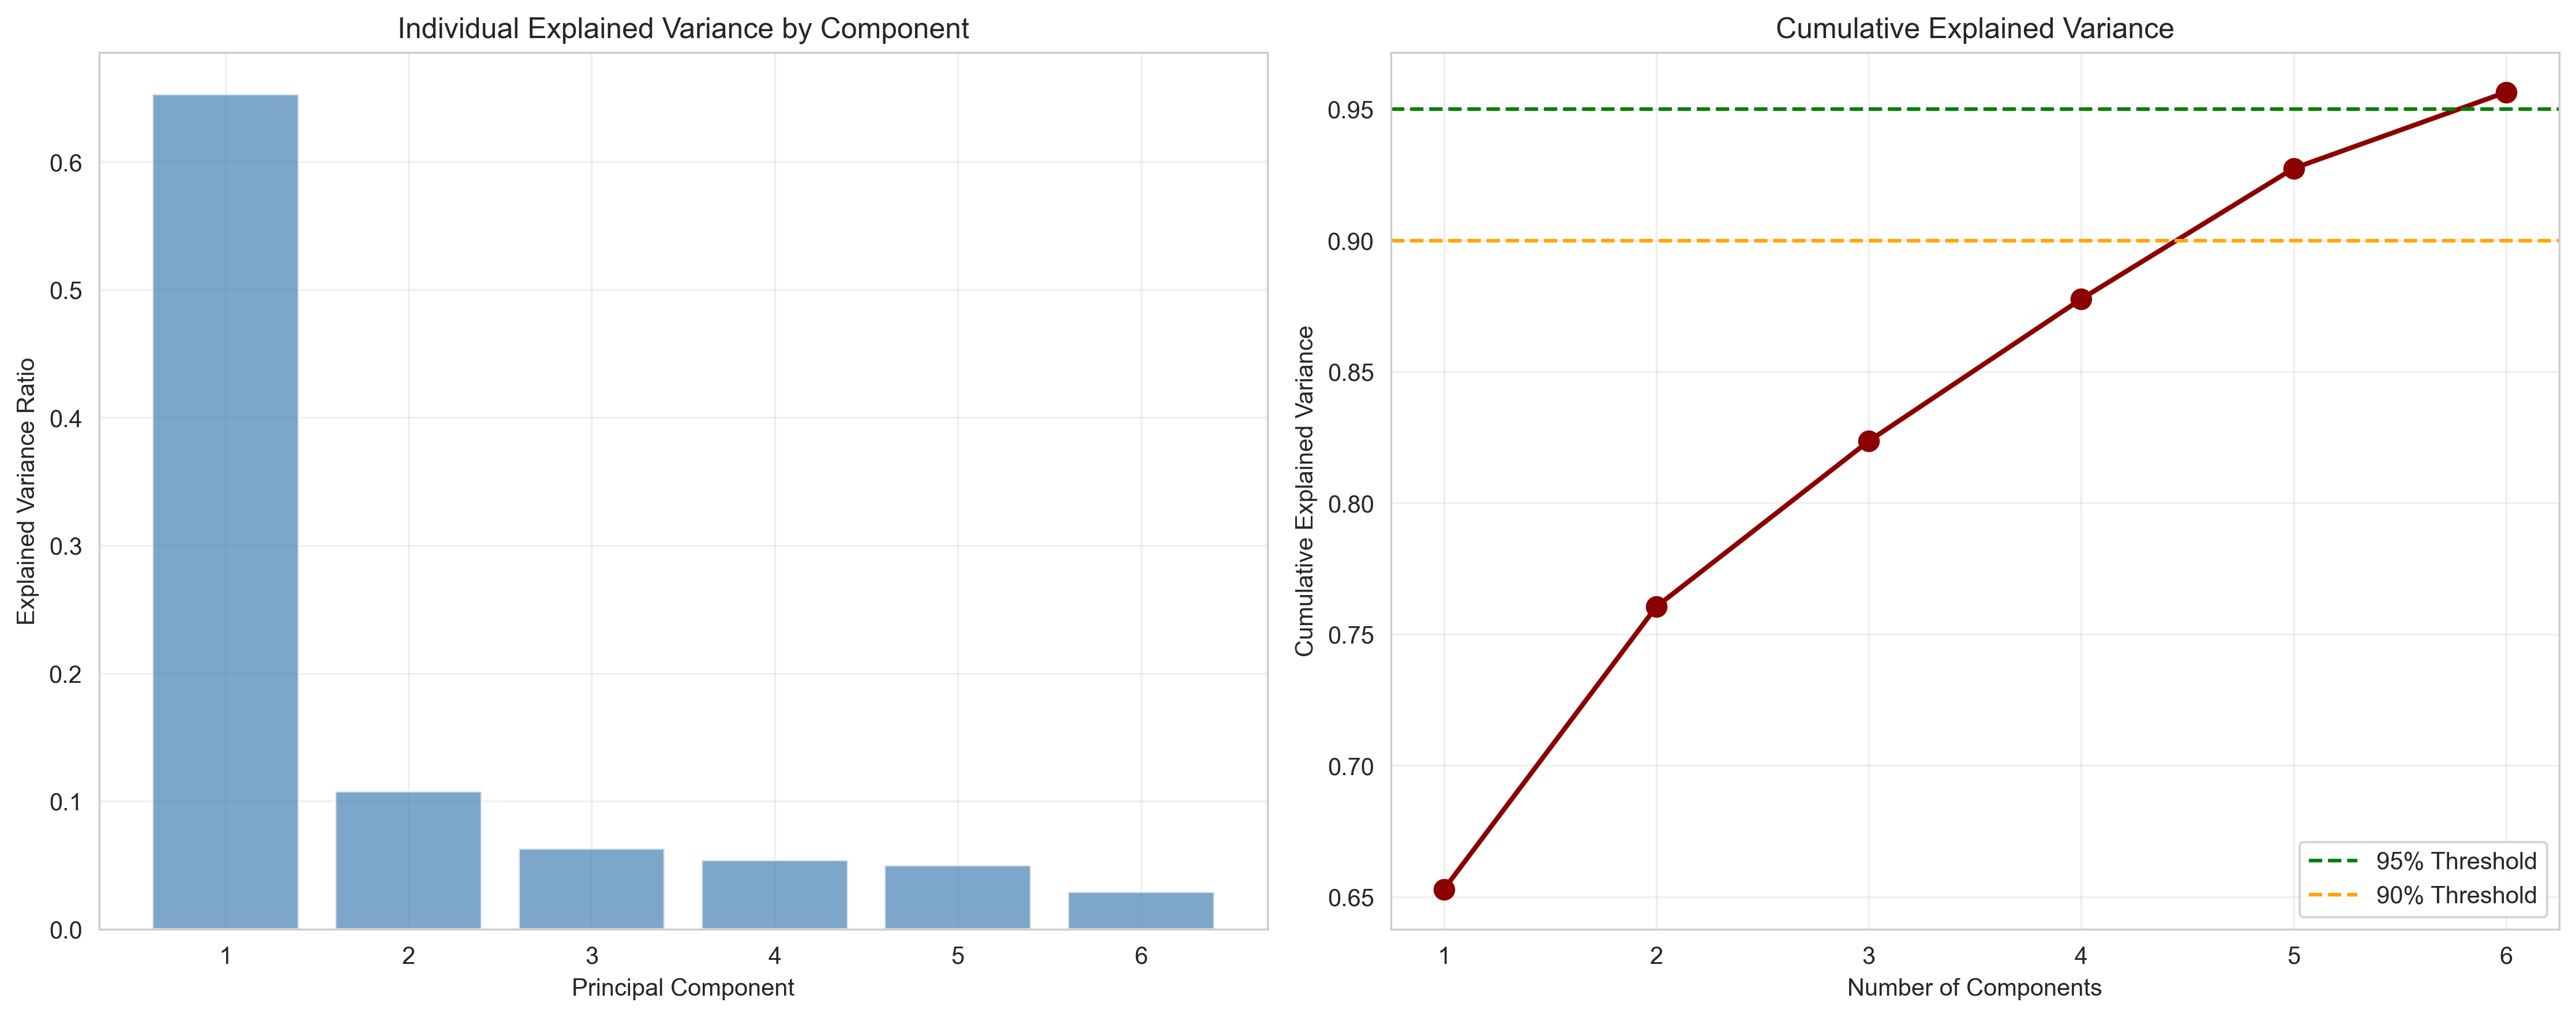
\includegraphics[width=0.9\textwidth]{../outputs/figures/explained_variance.png}
\caption{PCA explained and cumulative variance. Ten components retain 95.05\% of variance. The first component explains 33.9\% alone, indicating a dominant mode of variation.}
\label{fig:pca_variance}
\end{figure}

\begin{figure}[ht]
\centering
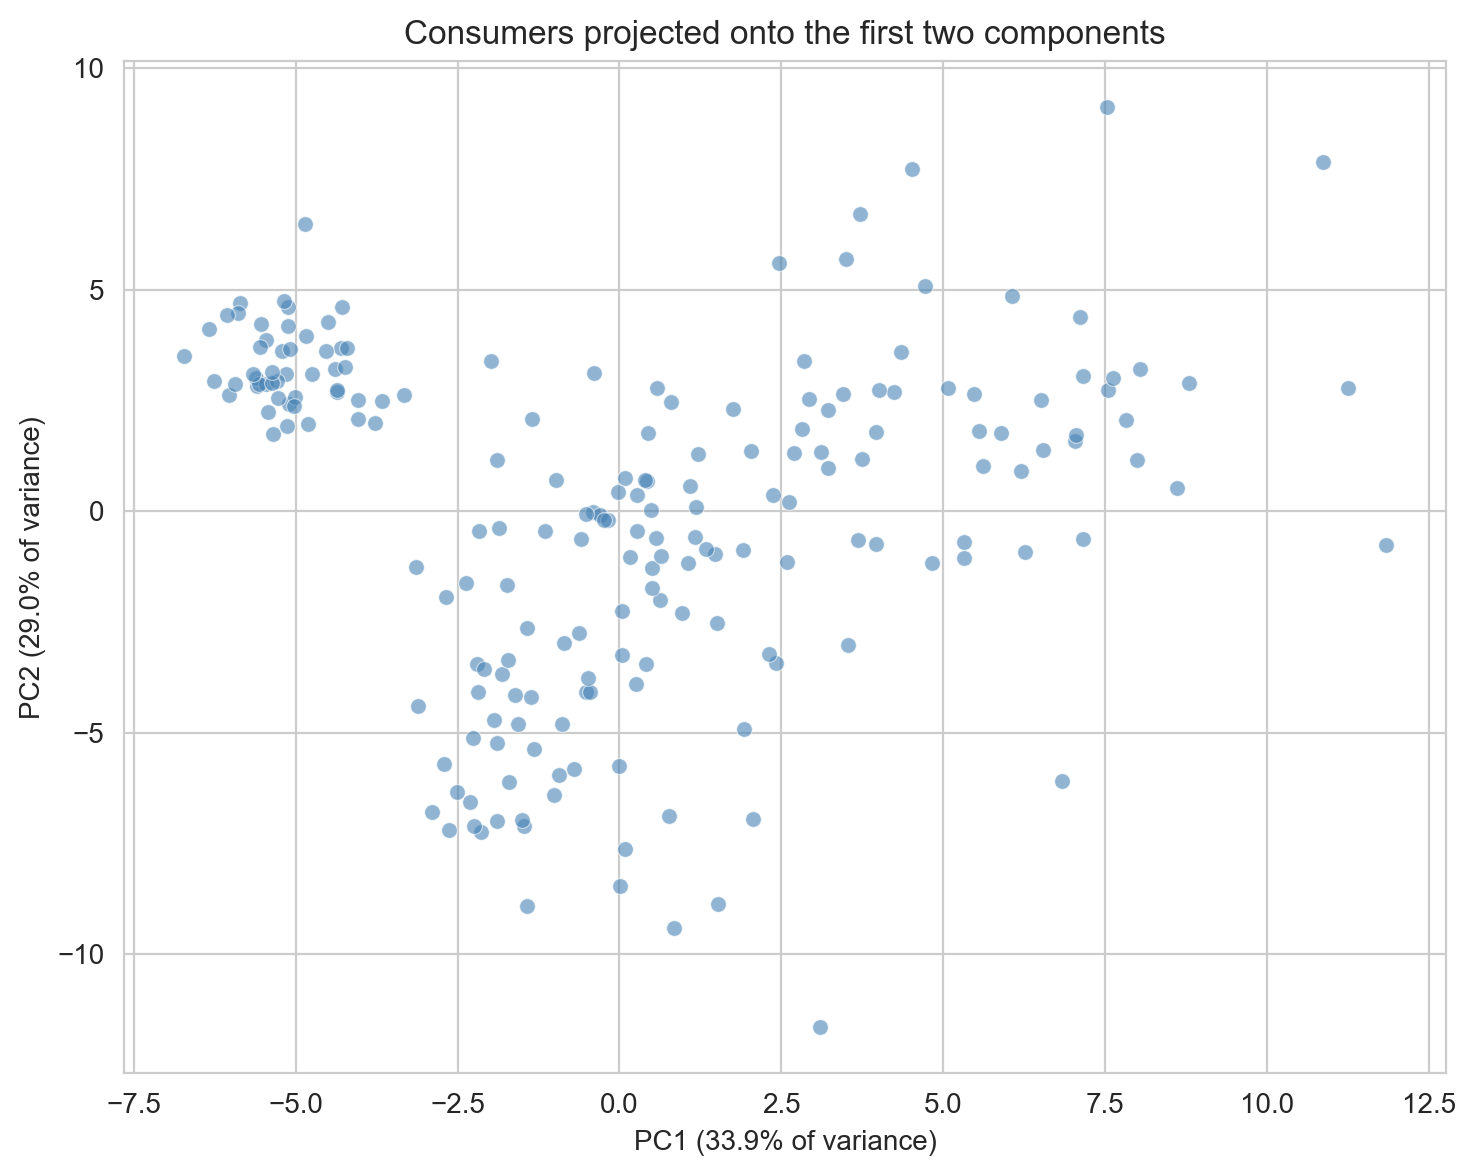
\includegraphics[width=0.8\textwidth]{../outputs/figures/pca_projection_2d.png}
\caption{\rev{PC1 vs PC2 projection of consumers colored by cluster assignment. The four clusters show separation in the principal component space, with PC1 capturing profile shape variation and PC2 capturing day/night balance.}}
\label{fig:pca_projection}
\end{figure}

\begin{figure}[ht]
\centering
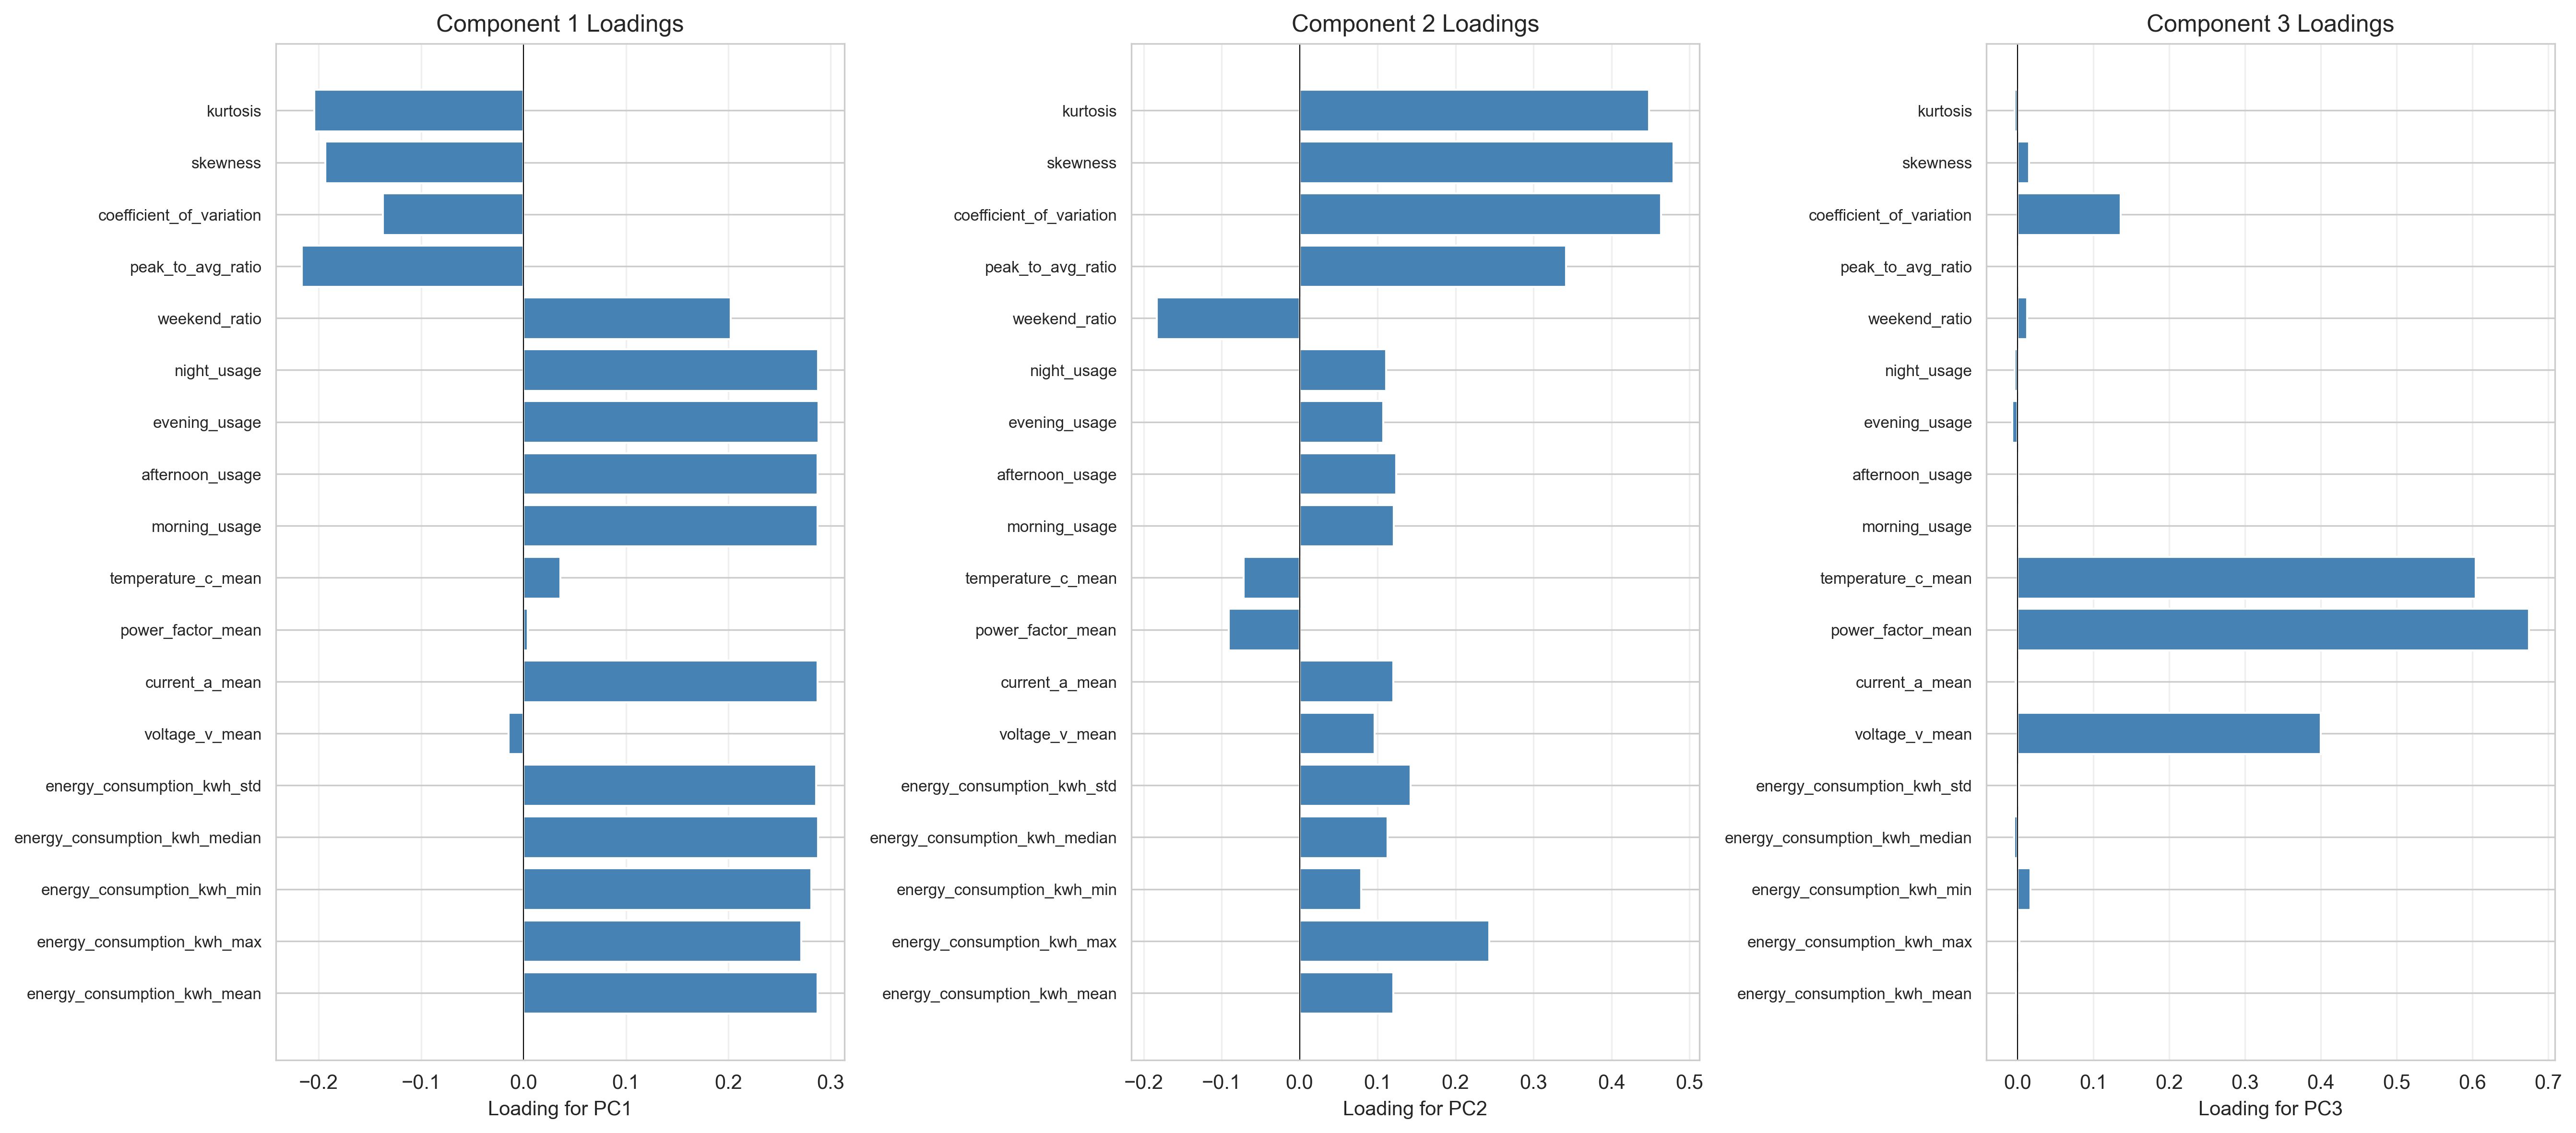
\includegraphics[width=0.9\textwidth]{../outputs/figures/component_loadings.png}
\caption{\rev{PCA loadings heatmap showing correlations between original features and principal components. Darker colors indicate stronger correlations. The heatmap confirms PC1 is dominated by profile shape features, PC2 by day/night balance, and PC3 by morning patterns.}}
\label{fig:pca_loadings}
\end{figure}

\textbf{Top PC Interpretations (via loadings):}
\begin{itemize}
    \item \textbf{PC1} (profile shape): profile\_ramp +0.92, peak\_concentration +0.88, harmonic\_2\_amplitude +0.88
    \item \textbf{PC2} (day/night balance): night\_day\_ratio +0.92, afternoon\_share -0.87
    \item \textbf{PC3} (morning pattern): hour\_7\_shape +0.87, hour\_8\_shape +0.87
    \item \textbf{PC4} (evening timing): hour\_17\_shape +0.56, hour\_18\_shape +0.54
    \item \textbf{PC5} (weekend behavior): weekend\_ratio -0.51, haar\_detail\_l3 +0.54
\end{itemize}

These interpretations confirm PCA captures complementary behavioral dimensions: overall profile shape, diurnal balance, specific hour patterns, and weekend effects.

\subsection{Selection of Number of Clusters}

Algorithm~\ref{alg:kselection} applied to candidates K=2 to 10 yields the selection shown in Figure~\ref{fig:k_selection}.

\begin{figure}[ht]
\centering
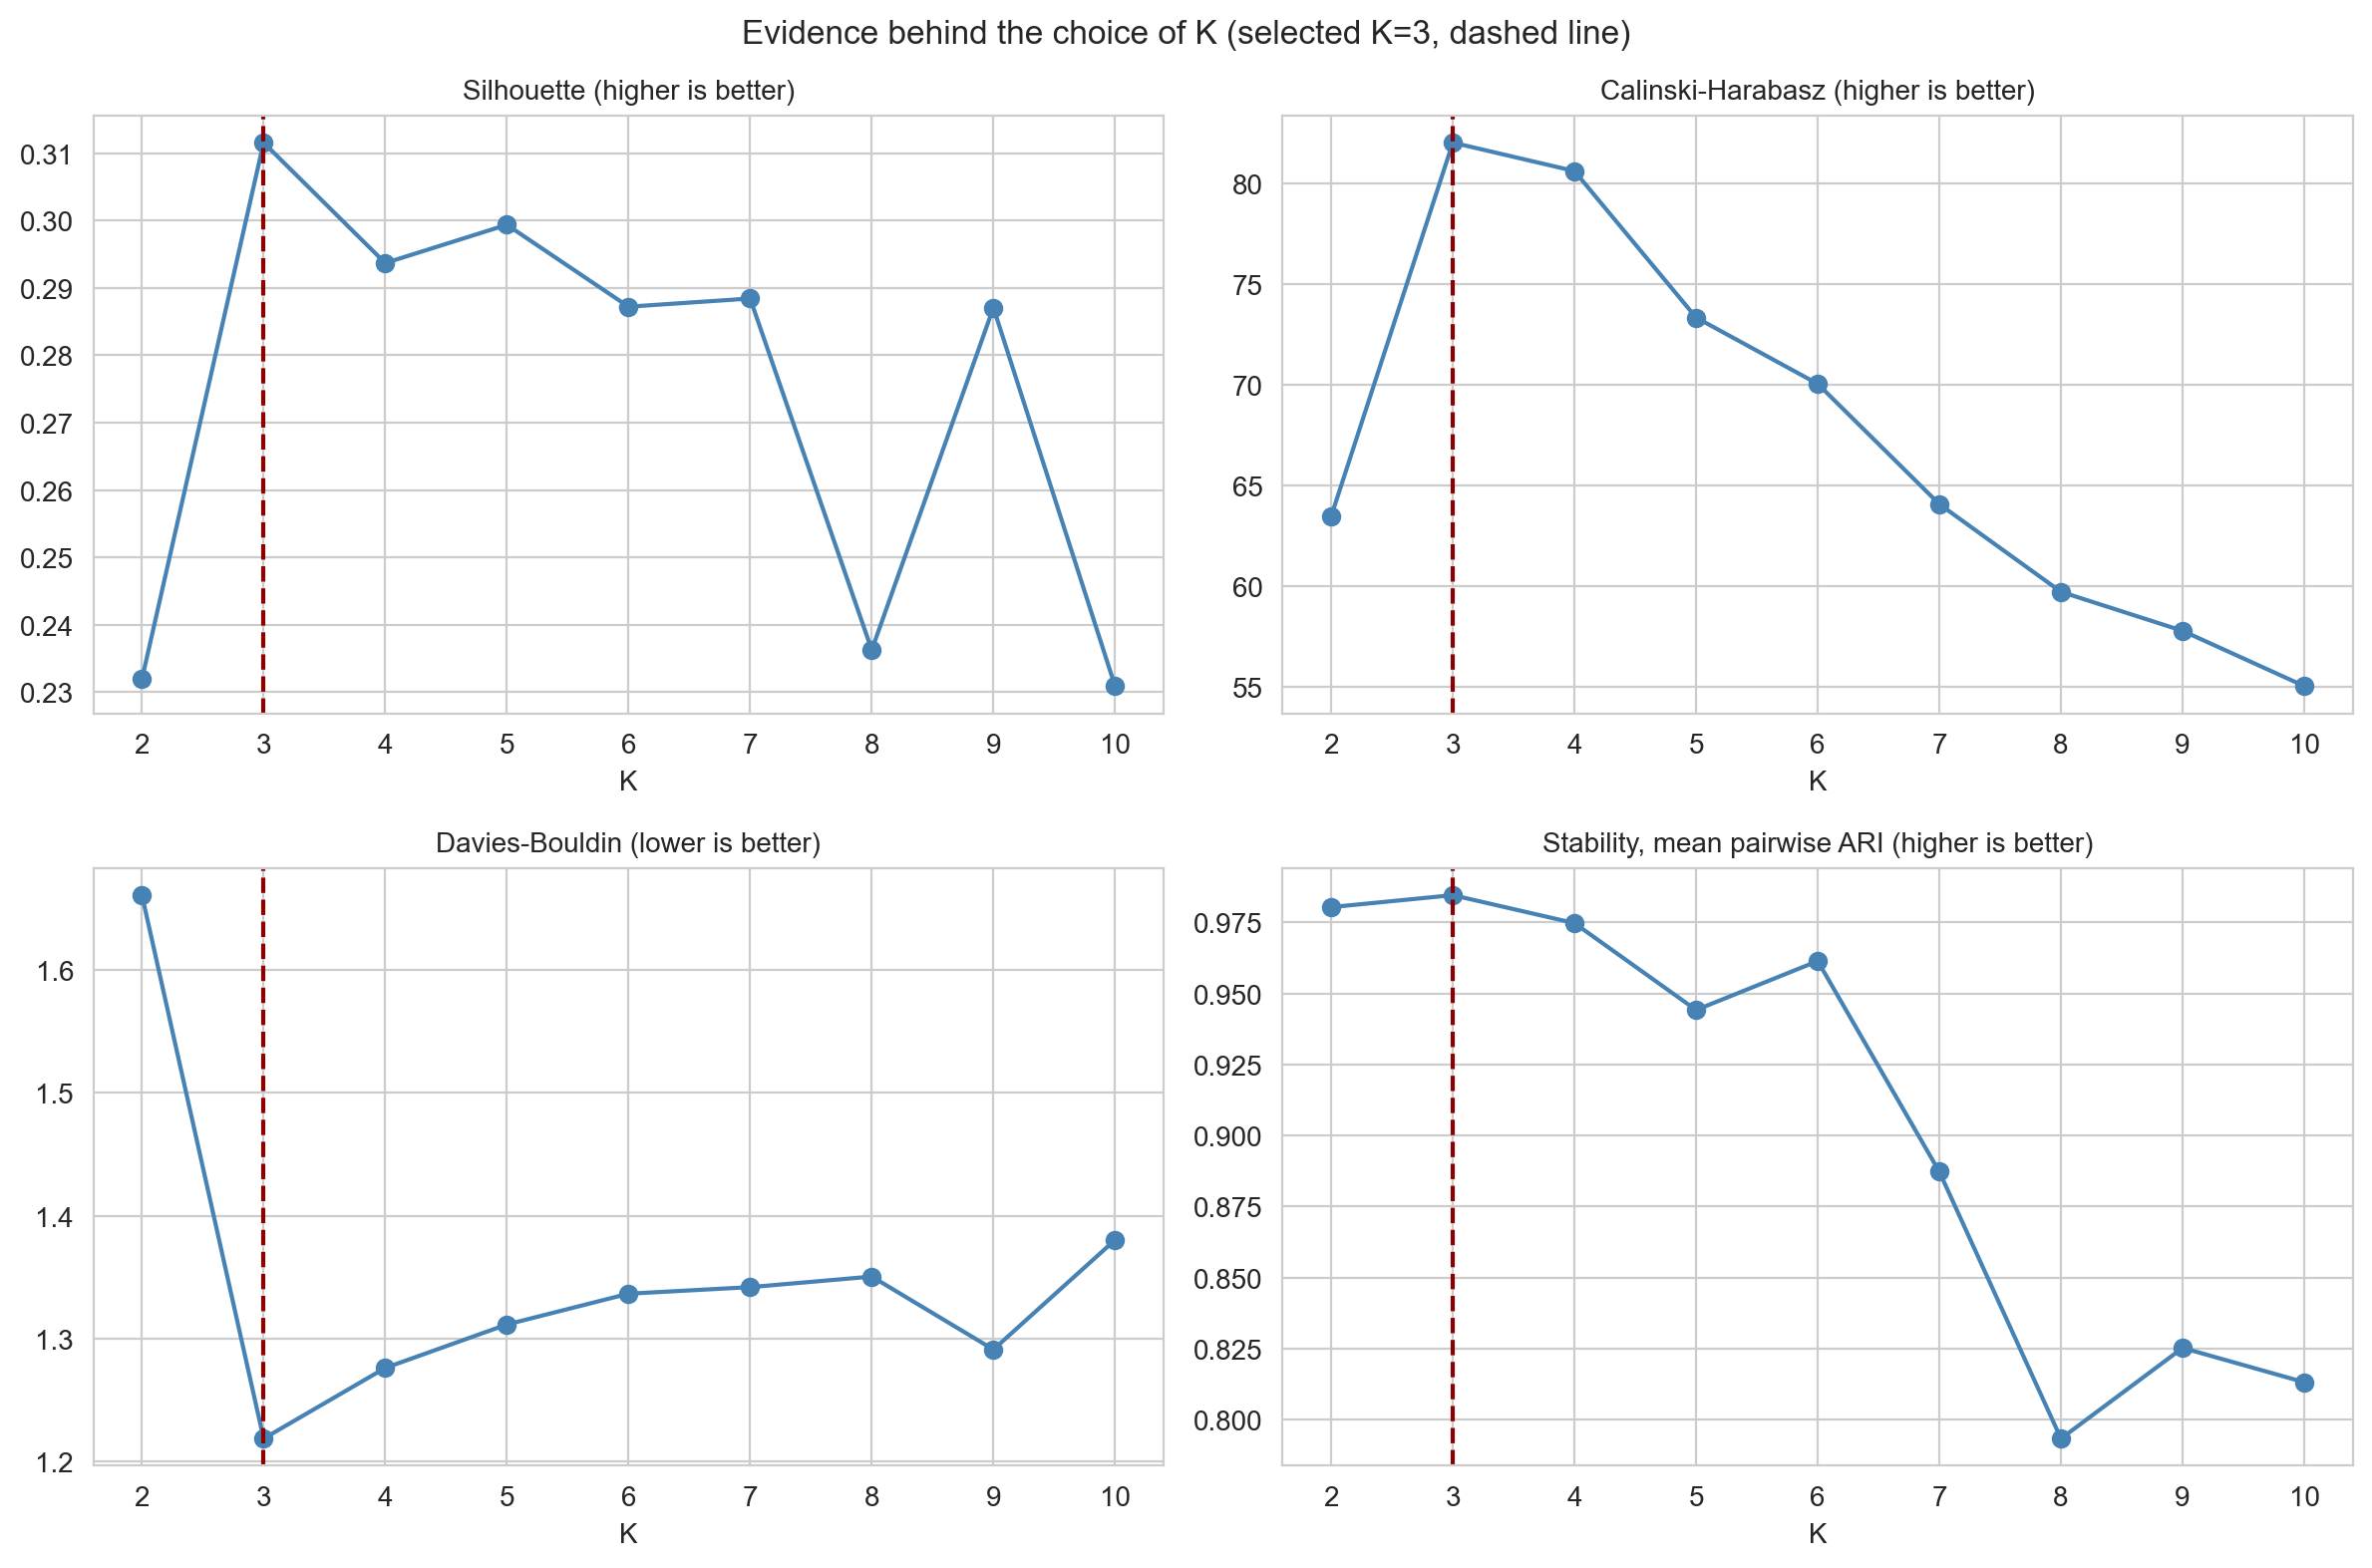
\includegraphics[width=0.9\textwidth]{../outputs/figures/k_selection_metrics.png}
\caption{K-selection metrics sweep. (a) Silhouette peaks at K=5 (0.335), (b) Calinski-Harabasz increases with K, (c) Davies-Bouldin minimized at K=4, (d) Composite score maximized at K=4. The evidence-based rule selects K=4.}
\label{fig:k_selection}
\end{figure}

\textbf{Selection Outcome:} K=4 selected with composite score 0.944. K=5 has marginally higher silhouette (0.335 vs 0.328) but lower composite (0.821). No other K within 0.05 tolerance, so parsimony rule not invoked. K=7-10 rejected for producing sub-5\% clusters.

\subsection{Clustering Results}

The four clusters exhibit semantically coherent behavioral patterns summarized in Table~\ref{tab:cluster_profiles}.

\begin{table}[ht]
\centering
\small
\caption{Cluster Profiles (K=4, Flagship)}
\label{tab:cluster_profiles}
\begin{tabular}{@{}lcccc@{}}
\toprule
Characteristic & Cluster 0 & Cluster 1 & Cluster 2 & Cluster 3 \\
\midrule
Size (N) & 39 & 52 & 47 & 62 \\
Share (\%) & 19.5 & 26.0 & 23.5 & 31.0 \\
Peak hour & 13:00 & 19:00 & 20:00 & 19:00 \\
Evening share & 0.212 & 0.258 & \textbf{0.380} & 0.299 \\
Afternoon share & \textbf{0.357} & 0.271 & 0.229 & 0.310 \\
Weekend ratio & \textbf{0.747} & 0.952 & 1.026 & \textbf{1.313} \\
Peak-to-avg & 8.83 & \textbf{4.92} & \textbf{11.32} & 9.45 \\
CV & 0.620 & \textbf{0.302} & 0.705 & 0.596 \\
\midrule
Assigned name & Midday- & Flat & Evening- & Evening- \\
 & Peaking & All-Day & Peaking & Peaking \\
 & Weekday- &  &  & Weekend- \\
 & Heavy &  &  & Heavy \\
\bottomrule
\end{tabular}
\end{table}

\begin{figure}[ht]
\centering
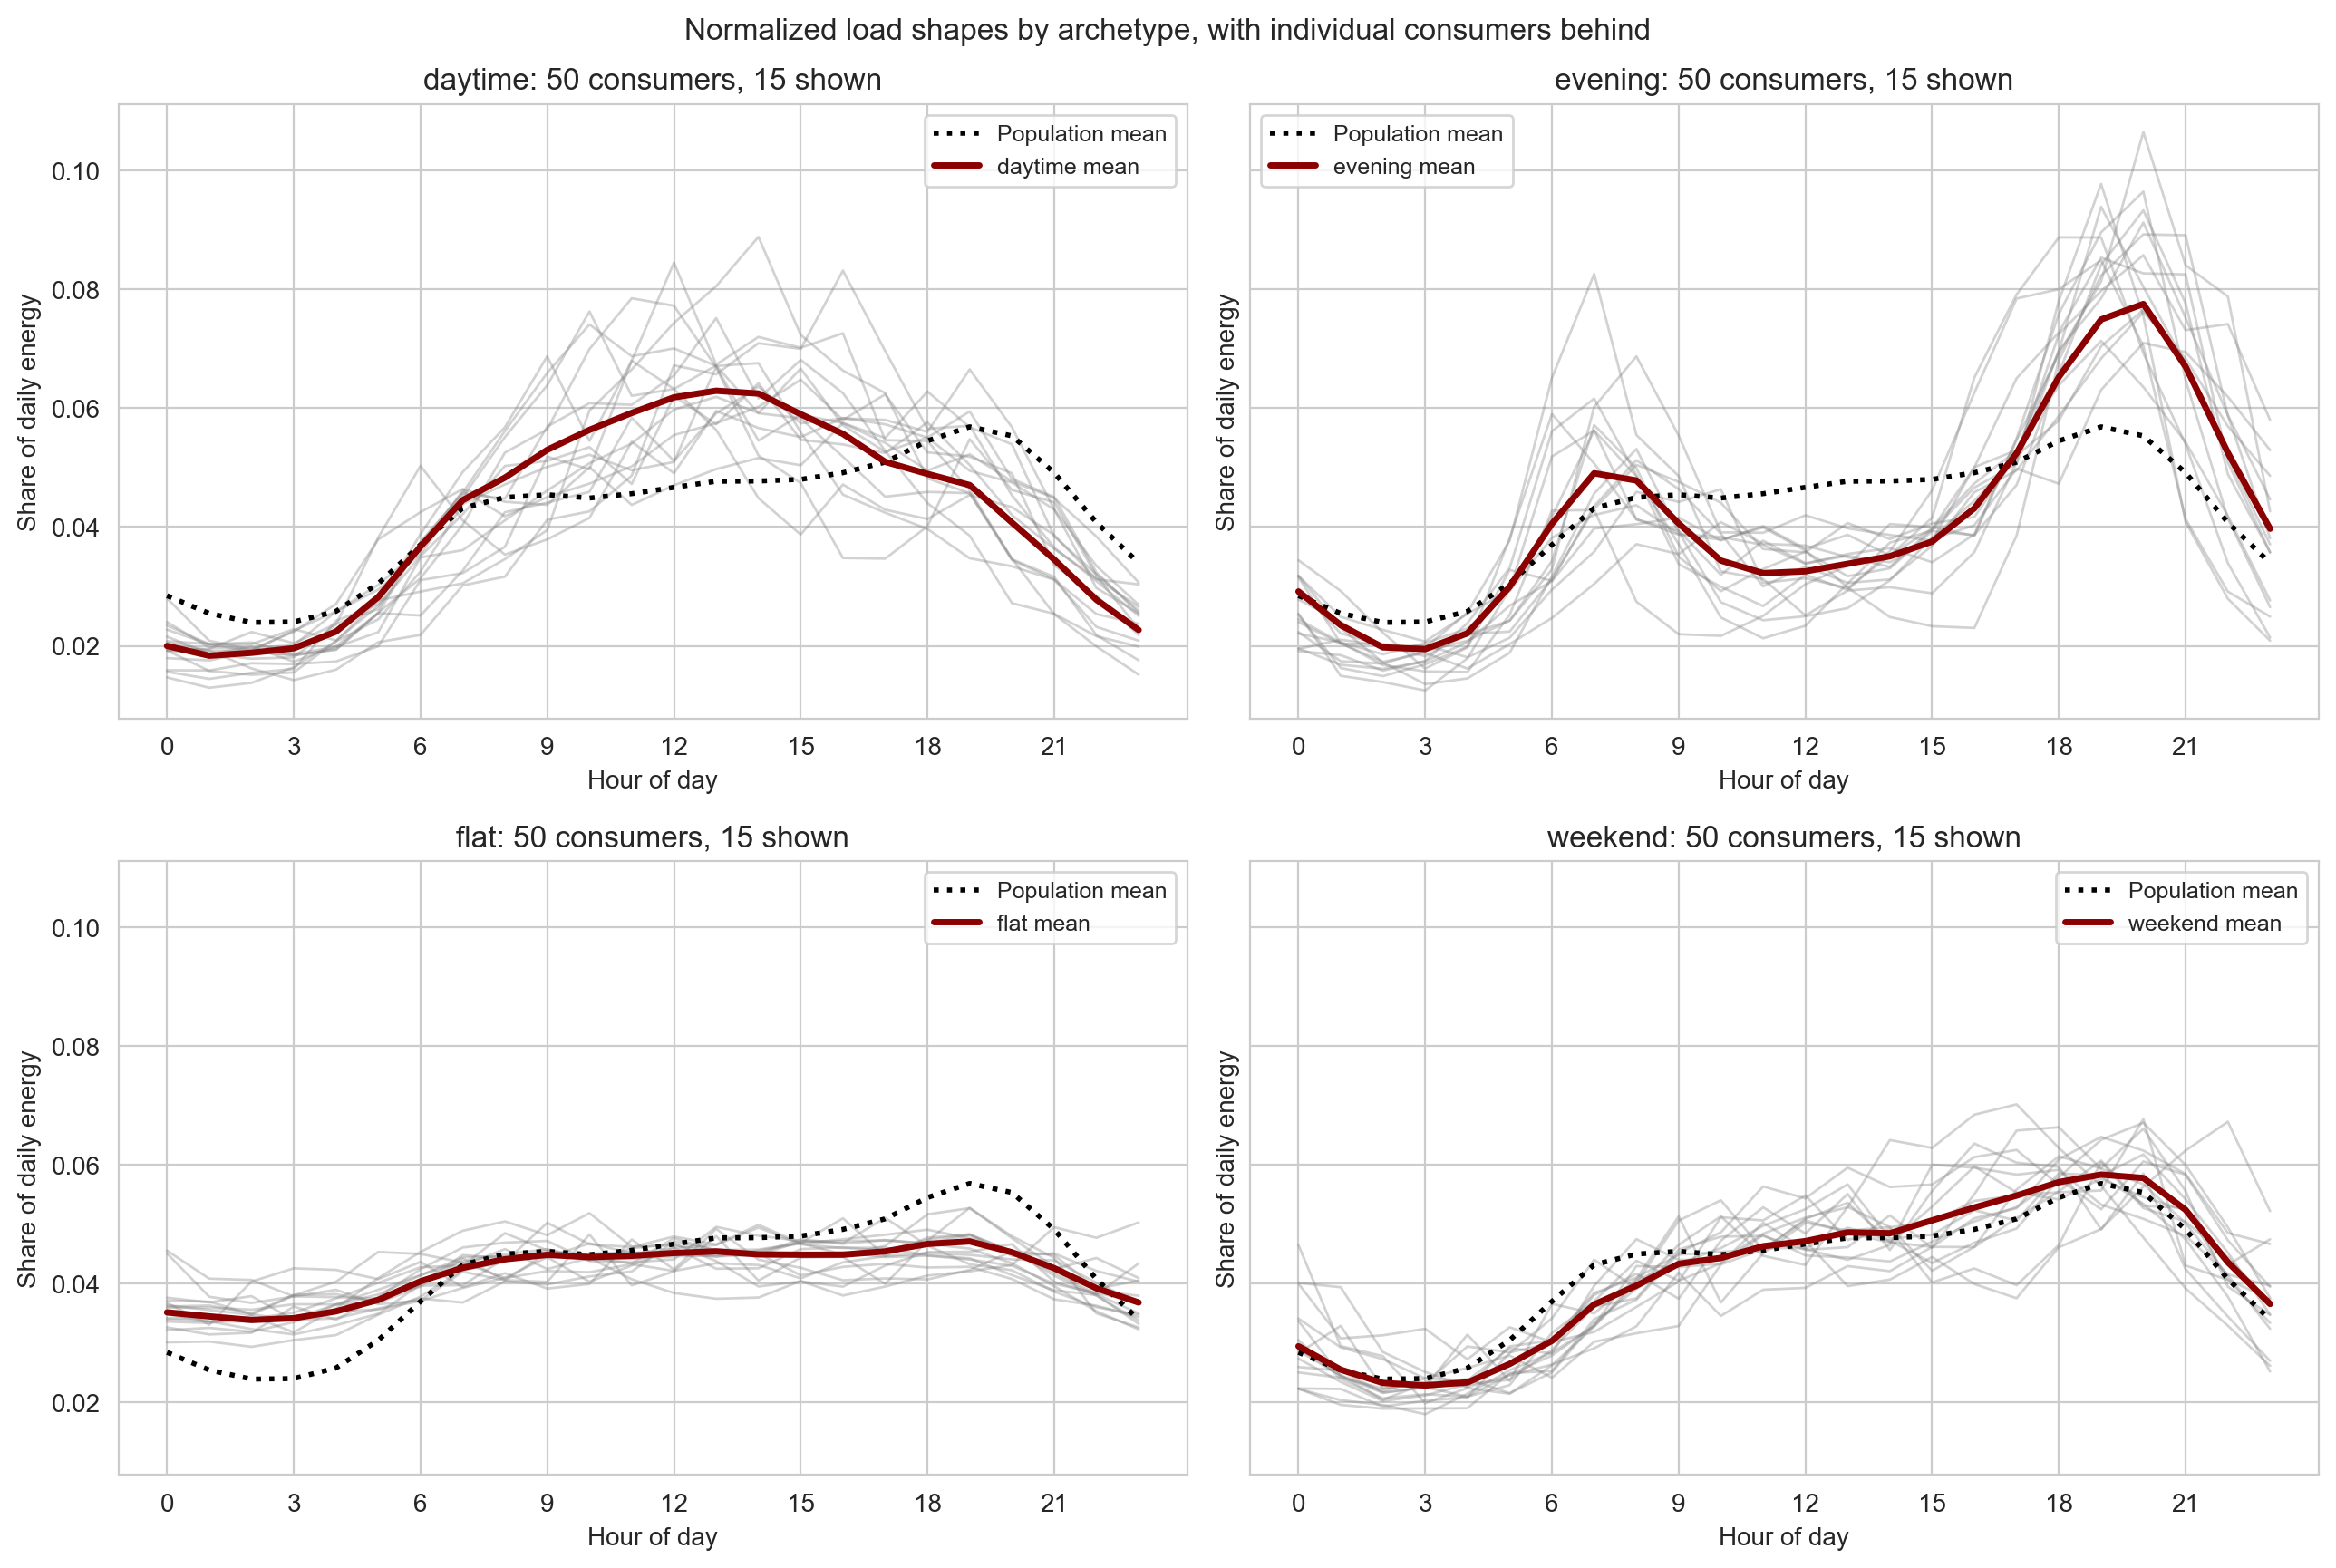
\includegraphics[width=0.9\textwidth]{../outputs/figures/archetype_profiles.png}
\caption{Cluster average 24-hour load profiles. Clusters differ primarily in timing (midday vs evening peaks) and weekend behavior (depressed vs elevated), not in magnitude.}
\label{fig:cluster_profiles}
\end{figure}

\textbf{Observations:}
\begin{itemize}
    \item \textbf{Cluster 0} (Midday-Peaking Weekday-Heavy): Afternoon peak (13:00), elevated afternoon share (0.357), depressed weekend ratio (0.747)
    \item \textbf{Cluster 1} (Flat All-Day): Lowest peak-to-average (4.92), lowest CV (0.302), near-uniform distribution
    \item \textbf{Cluster 2} (Evening-Peaking): Highest evening share (0.380), highest peak-to-average (11.32), concentrated evening demand
    \item \textbf{Cluster 3} (Evening-Peaking Weekend-Heavy): Evening peak with elevated weekend ratio (1.313)
\end{itemize}

\textbf{Mean Consumption Context:} Mean kWh/record for clusters [1.30, 1.38, 1.38, 1.32] vs population 1.35---approximately uniform, confirming magnitude does not drive clustering.

\subsection{Validation and Ground Truth Recovery}

Comparing recovered clusters against hidden behavioral archetypes (never used during modeling):

\begin{figure}[ht]
\centering
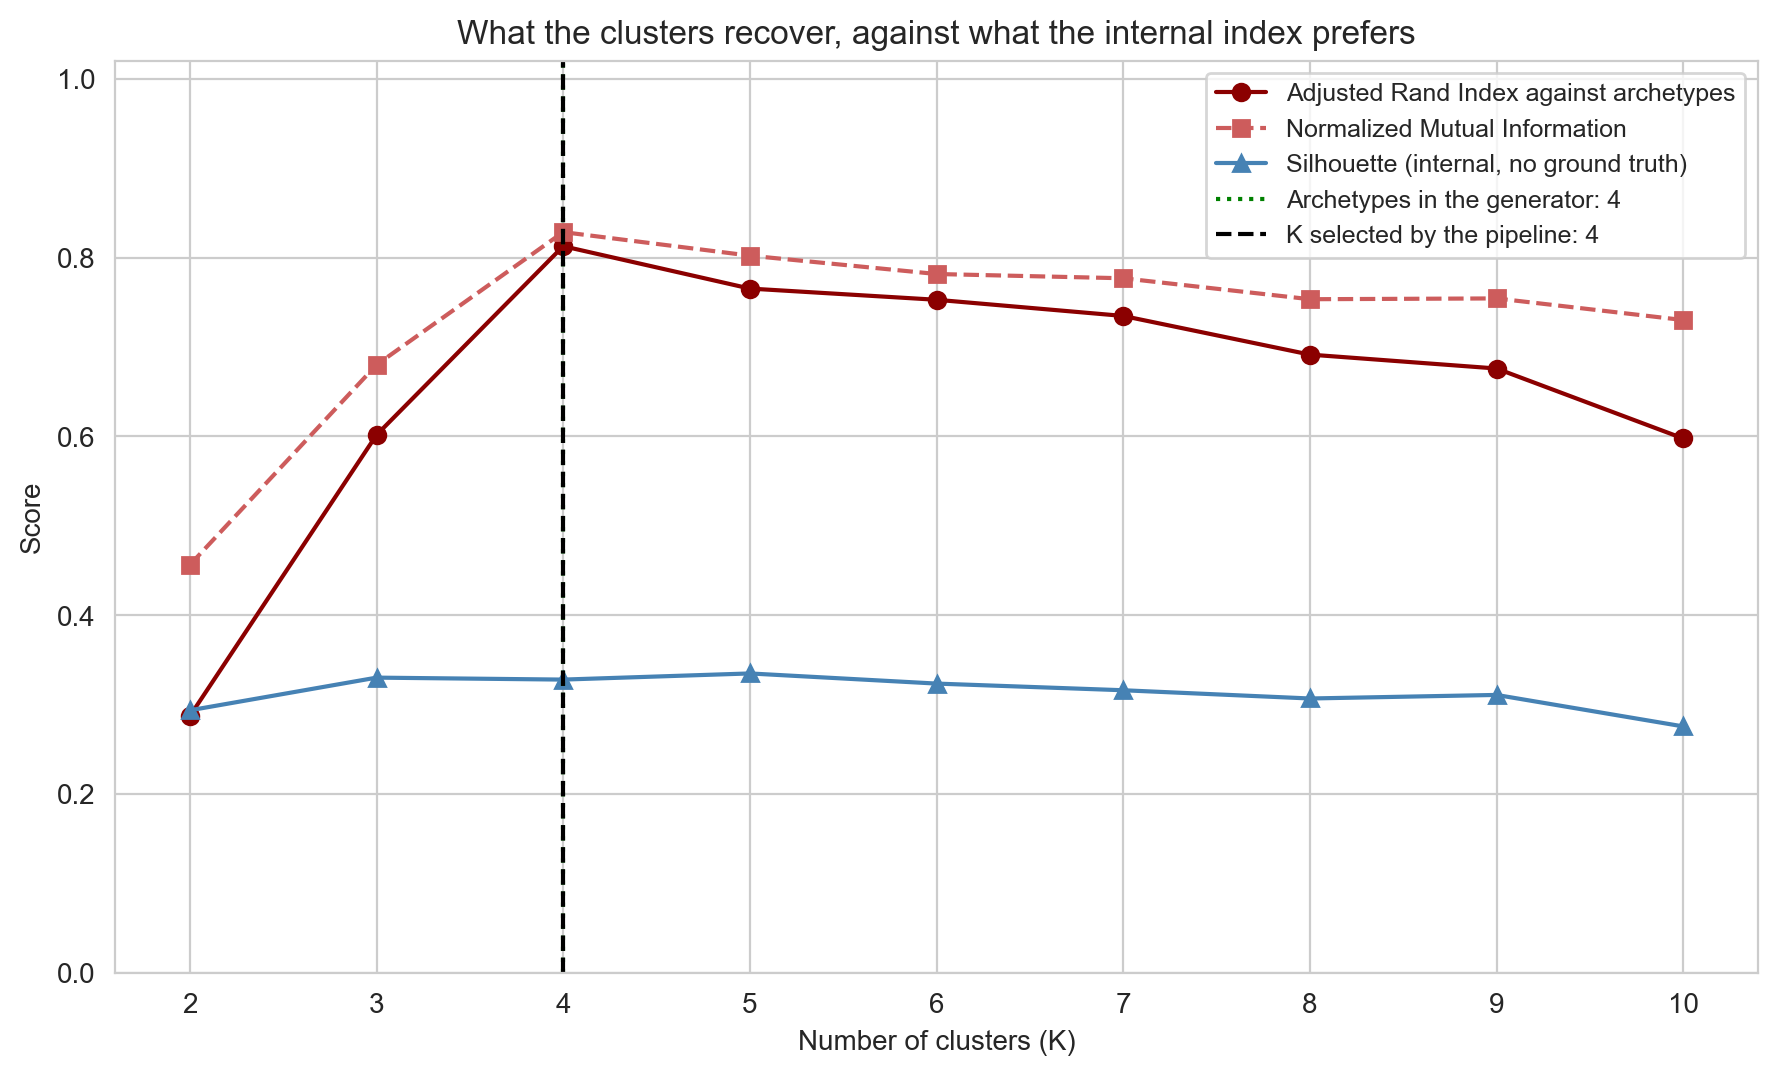
\includegraphics[width=0.8\textwidth]{../outputs/figures/archetype_recovery.png}
\caption{Ground-truth recovery on the synthetic flagship dataset: ARI and NMI versus K. Both metrics peak at K=4 (ARI=0.813, NMI=0.828), the K selected without access to archetype labels in this run. This single result does not establish that the selection rule will recover the true K on other datasets.}
\label{fig:recovery}
\end{figure}

\textbf{Key Finding:} ARI peaks at K=4 (0.813), which is also the K selected by the internal rule on this synthetic run. This is evidence of alignment for this controlled dataset, not proof that internal selection generally identifies a true K.

\textbf{Confusion Matrix at K=4:} Three archetypes recover near-perfectly (evening 47/50, flat 50/50, weekend 49/50). Daytime archetype splits: 39/50 in Cluster 0, 10/50 in Cluster 3, reflecting behavioral overlap between midday-peaking and evening-peaking patterns when weekend behavior differs.

\subsection{Stability and Robustness Results}

\subsubsection{Multi-Seed Stability}

Refitting K-means at K=4 with 10 random seeds yields:
\begin{itemize}
    \item Mean pairwise ARI: 0.995 $\pm$ 0.007
    \item Min ARI: 0.974
    \item Assignment agreement: 0.998
\end{itemize}

\textbf{Interpretation:} Partition is highly robust across initializations. Near-perfect stability (ARI $>$ 0.99) indicates clustering captures real structure, not random artifacts.

\subsubsection{Temporal Stability}

Quarterly segments re-analyzed independently:

\begin{figure}[ht]
\centering
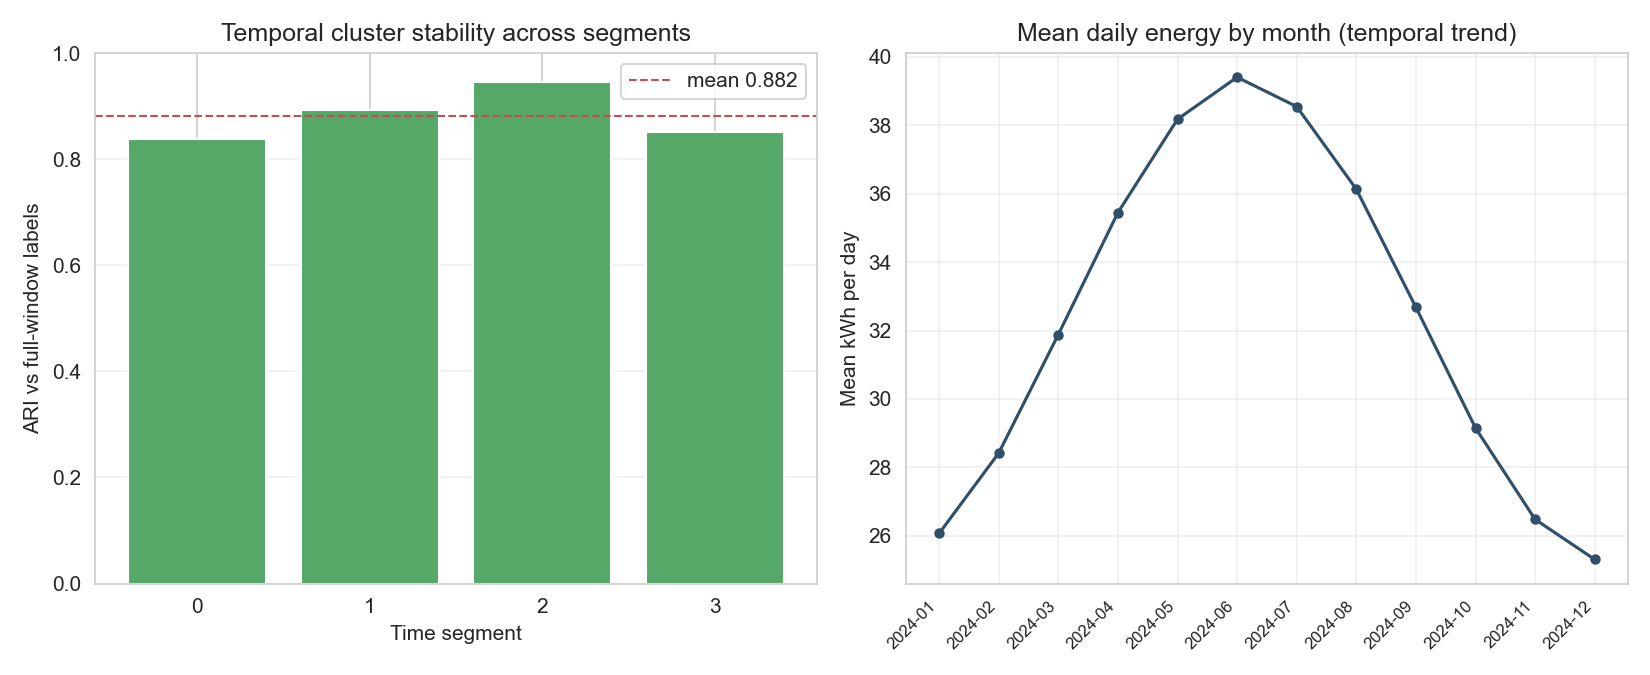
\includegraphics[width=0.8\textwidth]{../outputs/figures/longitudinal_cluster_stability.png}
\caption{Temporal stability across quarterly segments. All segments independently select K=4. Mean ARI vs full window is 0.882, demonstrating consumer groups persist across seasons despite magnitude variations.}
\label{fig:temporal_stability}
\end{figure}

\textbf{Observations:}
\begin{itemize}
    \item All segments independently select K=4, confirming evidence-based rule consistency
    \item High temporal ARI ($>$0.84 all quarters, mean 0.882) demonstrates consumer groups persist across seasons
    \item Q3 (summer) shows strongest alignment (0.946); Q1 (winter) weakest (0.838) but still strong
\end{itemize}

\textbf{Interpretation:} Behavioral groupings are stable properties of the modeled archetypes under the tested seasonal perturbations, not seasonal artifacts. Despite magnitude variations (monthly mean kWh: Jan 26.1 $\rightarrow$ Jun 39.4 $\rightarrow$ Dec 25.3), temporal patterns remain coherent.

\subsection{Unsupervised Analysis of UCI Client Data}
\label{sec:uci-results}

On the 104 active clients in the seeded 2012 sample, PCA retained 11 of 51 behavioral features (95.54\% cumulative variance). The K-selection procedure selected $K=2$: this was the only candidate in the tested range $K=2$--8 whose reference partition met the five-percent minimum-cluster-size rule. The elbow estimate was $K=4$, but those larger candidates contained clusters below the pre-specified size threshold. Thus, the selected value is the outcome of this heuristic and sample, not an estimate of a true number of behavioral groups. At $K=2$, silhouette was 0.466, Calinski--Harabasz was 37.6, and Davies--Bouldin was 0.908.

The eight fixed-seed K-means restarts produced identical partitions (mean pairwise ARI 1.000). In contrast, refitting the full feature/PCA/clustering pipeline independently in three equal-duration chronological windows produced mean pairwise ARI 0.288 (standard deviation 0.466 across the three window pairs). This low temporal agreement limits any claim that the full-year partition persists through the year. It also shows that restart stability alone is insufficient evidence of temporal robustness.

Table~\ref{tab:uci_cluster_profiles} and Figure~\ref{fig:uci_cluster_shapes} summarize the full-year partition descriptively. Cluster 0 (90 clients, 86.5\%) has a broad profile with more overnight energy share; Cluster 1 (14 clients, 13.5\%) has lower overnight share and greater daytime/afternoon share. Mean individual peak hour and other profile measures describe these sample clusters only. With no behavioral labels, these patterns cannot be interpreted as household routines or validated as useful customer segments.

\begin{table}[ht]
\centering
\small
\caption{Descriptive profiles for the full-year UCI client sample ($K=2$).}
\label{tab:uci_cluster_profiles}
\begin{tabular}{@{}lcc@{}}
\toprule
Measure & Cluster 0 & Cluster 1 \\
\midrule
Clients ($n$) & 90 & 14 \\
Share & 86.5\% & 13.5\% \\
Mean individual peak hour & 16.6 & 18.5 \\
Evening energy share & 0.282 & 0.334 \\
Afternoon energy share & 0.289 & 0.377 \\
Night energy share & 0.174 & 0.092 \\
Peak-to-average ratio & 2.33 & 2.83 \\
Coefficient of variation & 0.391 & 0.649 \\
Weekend ratio & 0.993 & 0.958 \\
\bottomrule
\end{tabular}
\end{table}

\begin{figure}[ht]
\centering
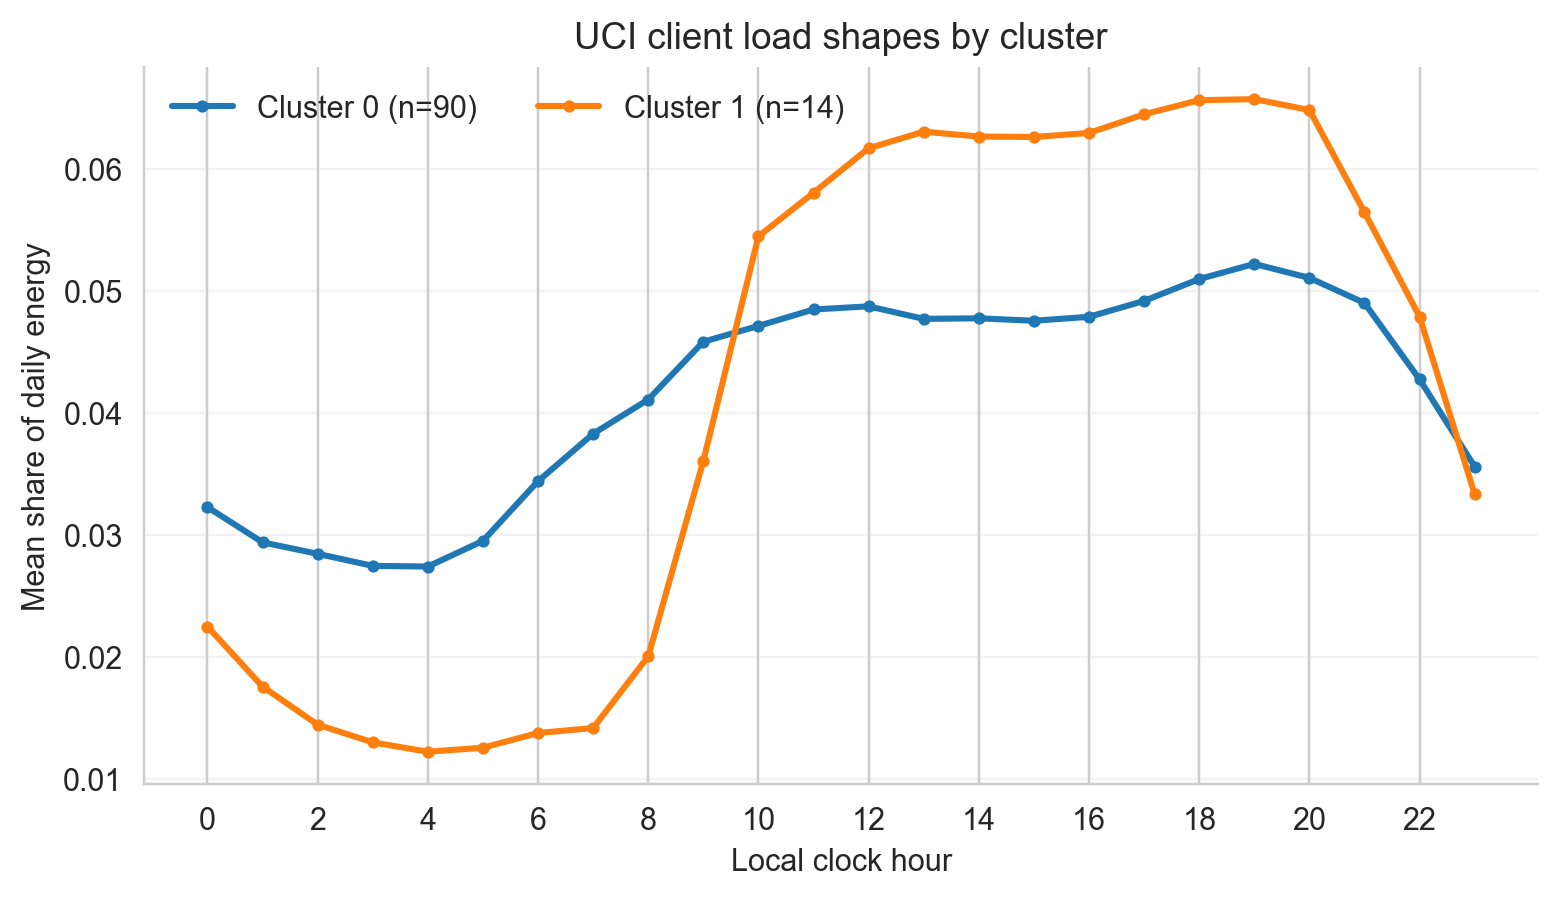
\includegraphics[width=0.9\textwidth]{../outputs/figures/real_world/cluster_load_shapes.png}
\caption{Mean normalized 24-hour load shape for each UCI client cluster. Each client's profile is normalized by its daily energy before aggregation; the figure is descriptive and does not imply ground-truth behavior.}
\label{fig:uci_cluster_shapes}
\end{figure}

\subsection{Feature Ablation}

Five feature sets compared on 30-day window with identical protocol:

\begin{figure}[ht]
\centering
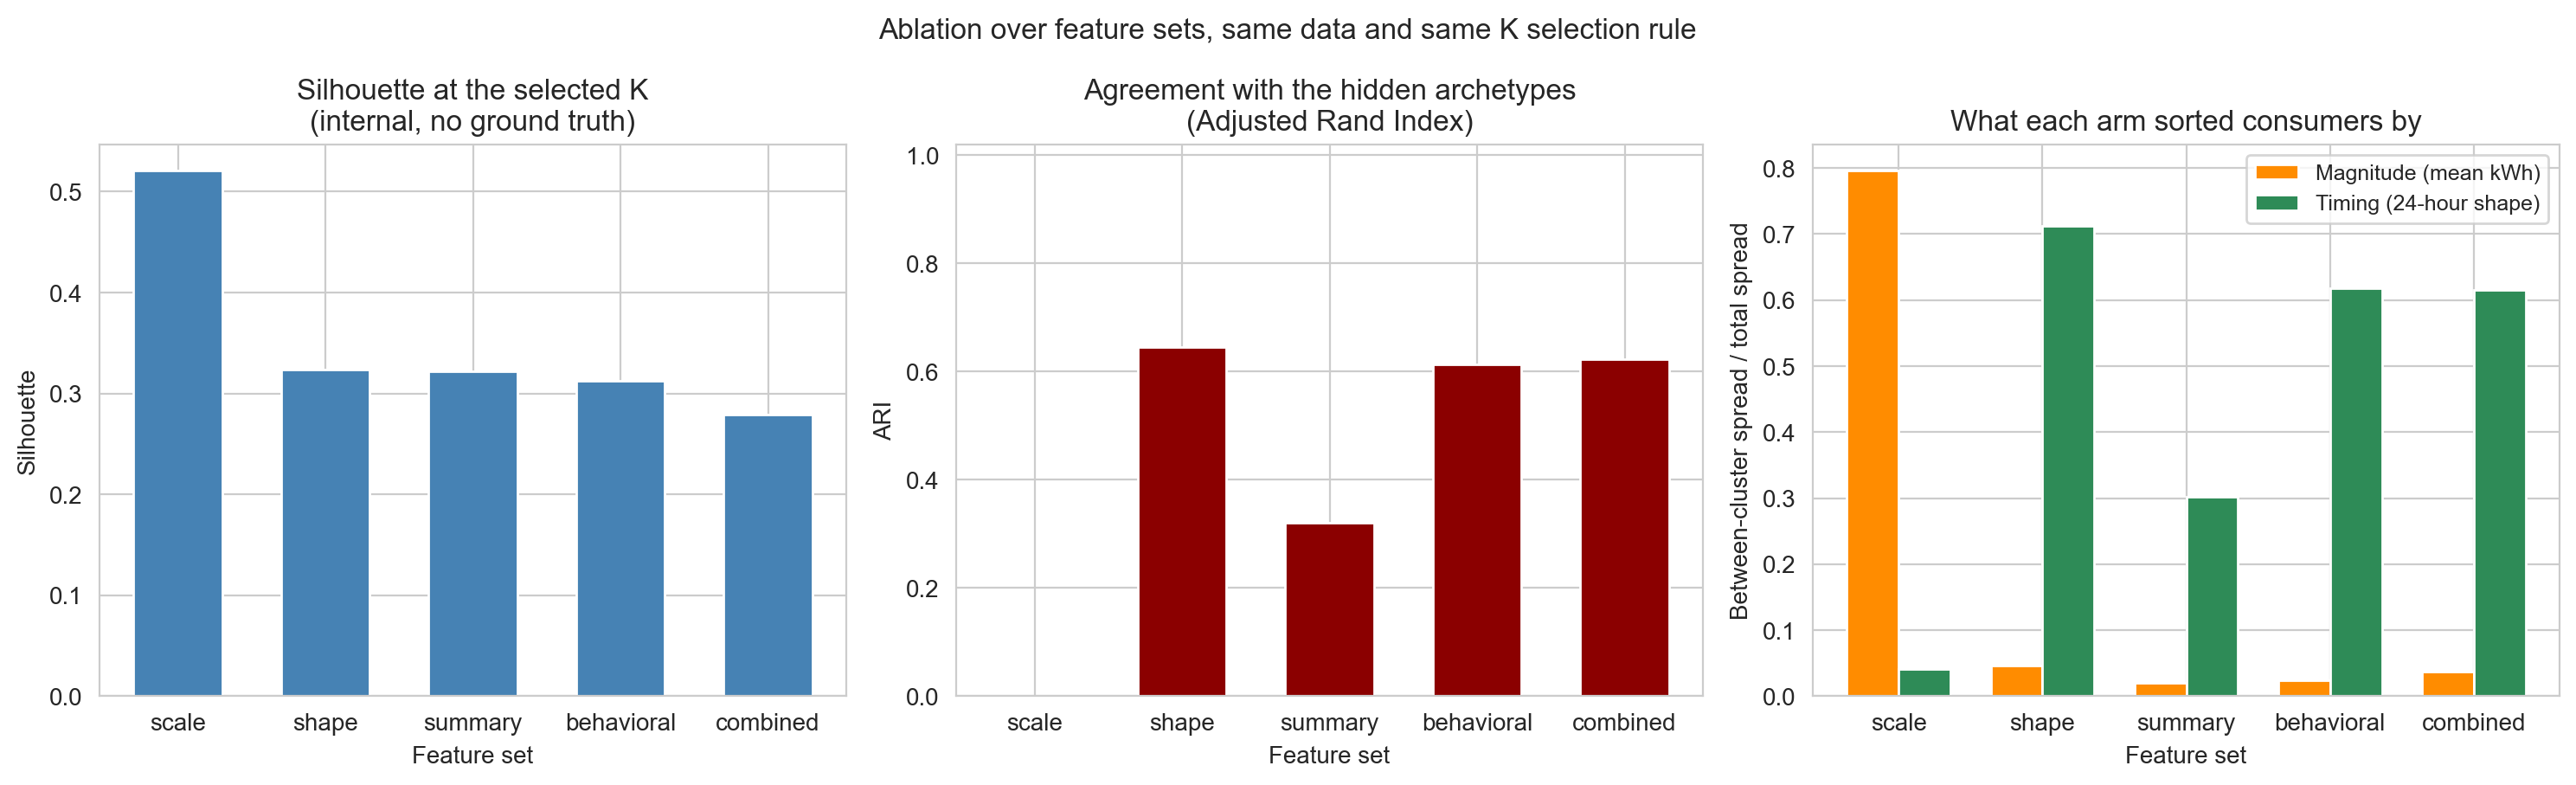
\includegraphics[width=0.9\textwidth]{../outputs/figures/ablation_comparison.png}
\caption{Ablation study: feature set comparison. (a) Scale features achieve highest silhouette (0.521) but (b) zero archetype recovery (ARI=-0.004). (c) All feature sets achieve high stability. This demonstrates internal metrics alone cannot validate behavioral segmentation.}
\label{fig:ablation}
\end{figure}

\textbf{Critical Finding:} Scale-only features achieve highest silhouette (0.521) but zero behavioral recovery (ARI -0.004). This demonstrates internal quality metrics alone cannot validate behavioral segmentation. High silhouette on magnitude simply confirms consumers with different totals are well-separated---but this is the wrong research question.

Behavioral and combined feature sets achieve similar recovery (0.614, 0.623), with behavioral slightly simpler (51 vs 58 features). Shape-only achieves 0.646, suggesting raw hourly bins carry strong signal, but behavioral descriptors add interpretability.

\subsubsection{Robustness Across 20 Datasets}

Twenty independent 30-day datasets (seeds 1-19, 42), five feature sets each:

\begin{figure}[ht]
\centering
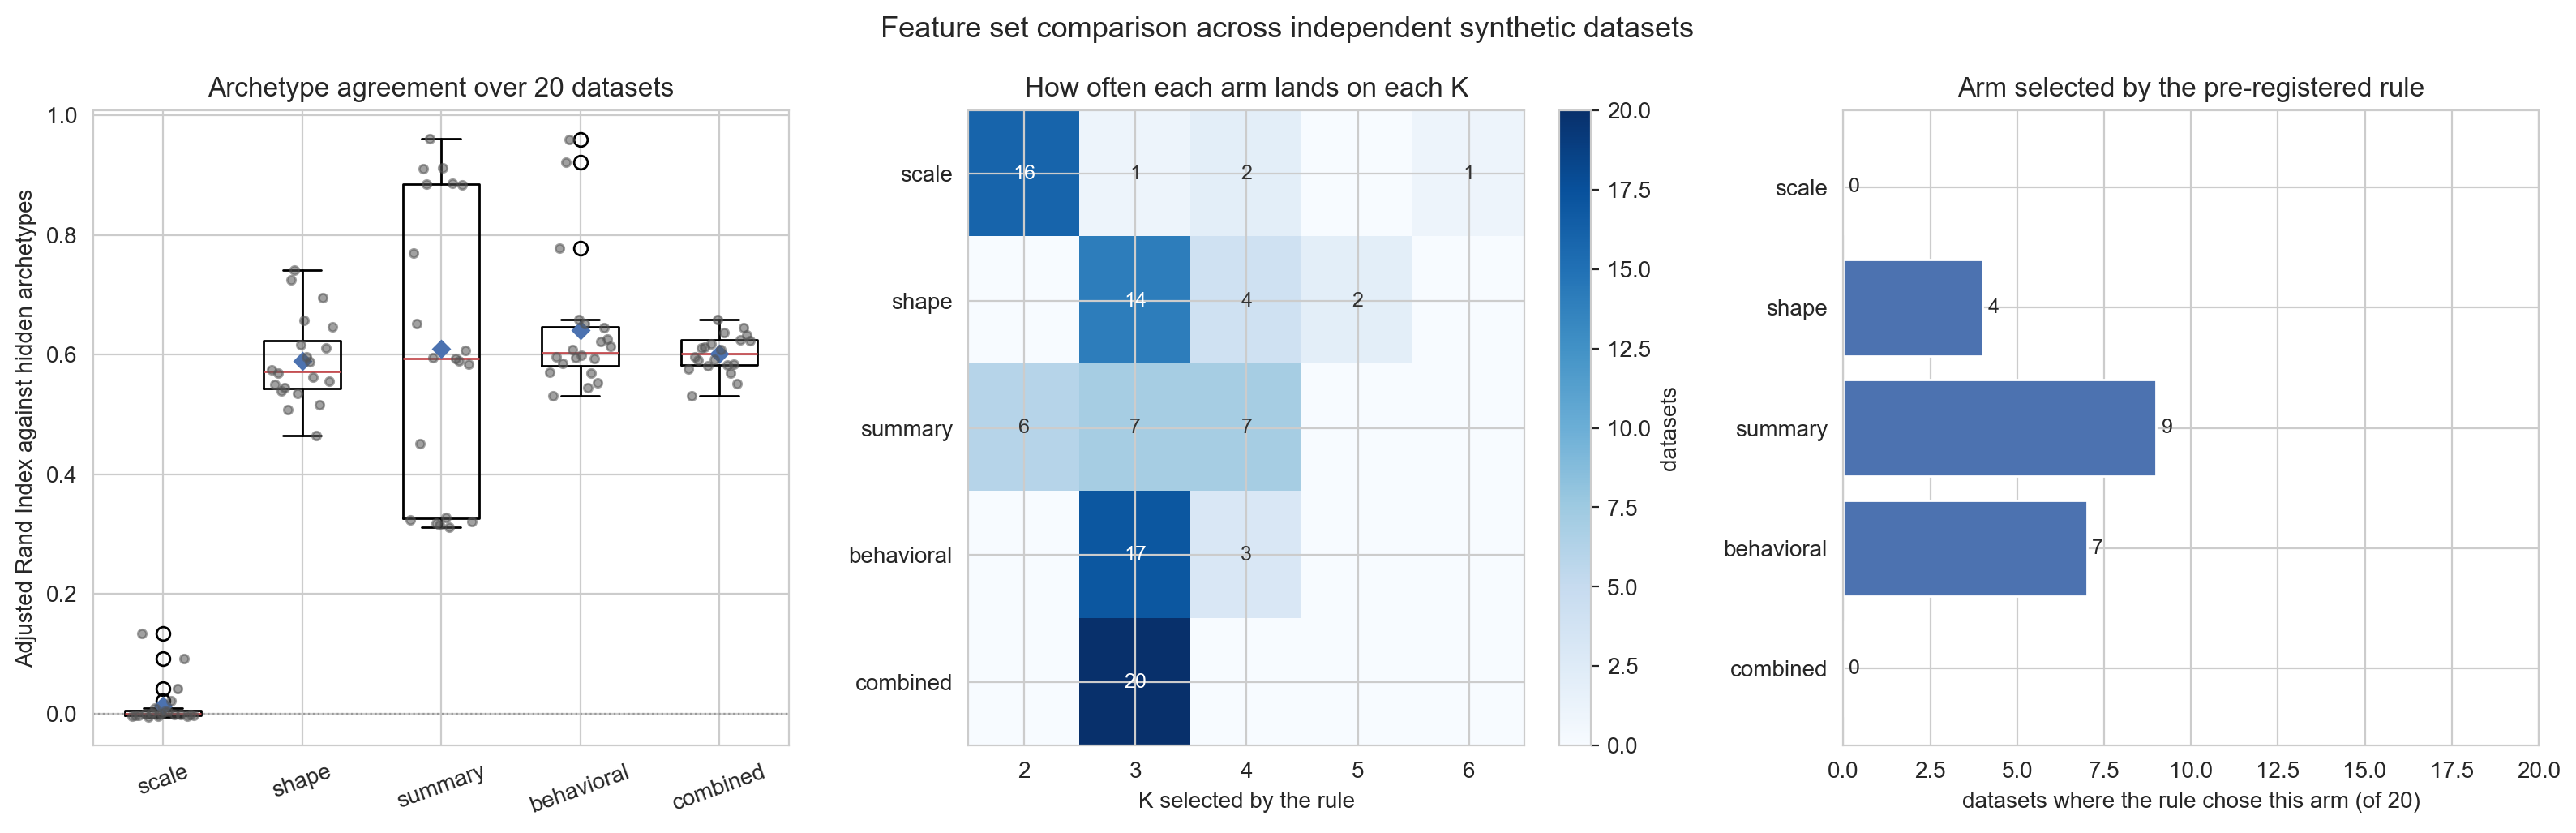
\includegraphics[width=0.8\textwidth]{../outputs/figures/seed_robustness.png}
\caption{Archetype ARI across 20 independently generated synthetic datasets. Behavioral features have mean recovery 0.641 ($\pm$0.115); scale features have mean recovery 0.013 ($\pm$0.036). An unadjusted paired permutation comparison of behavioral versus scale recovery gives $p=1.9\times10^{-6}$; this result applies to the tested synthetic generator.}
\label{fig:robustness}
\end{figure}

\textbf{Statistical Tests (Paired Permutation):}
\begin{itemize}
    \item Behavioral vs scale: unadjusted $p = 1.9 \times 10^{-6}$
    \item Behavioral vs shape: unadjusted $p = 0.123$; this does not establish equivalence or that the methods perform the same
\end{itemize}

\textbf{Interpretation:} The observed mean ARIs for behavioral, summary, and shape feature sets are close, but these comparisons do not establish equivalence. The behavioral representation is retained for its combination of scale-normalized design and feature-level interpretability; the synthetic experiment does not show that it is uniquely best.

For this synthetic generator, scale-only features consistently have near-zero archetype recovery (mean ARI $\approx$ 0.01) despite high silhouette. This result is specific to the tested generation and clustering setup.

% ============================================================================
% 6. DISCUSSION
% ============================================================================
\section{Discussion}
\label{sec:discussion}

\subsection{Principal Findings}

The synthetic and measured-data analyses support different, limited conclusions. Four findings emerge:

\textbf{1. Magnitude-Timing Separation Helps on the Tested Synthetic Data.} In the ablation study (Figure~\ref{fig:ablation}), magnitude-only features achieve near-zero archetype recovery (ARI -0.004) despite the highest internal silhouette (0.521). This shows that, for this generator and protocol, internal geometric quality does not imply recovery of the intended archetypes. The 51-feature behavioral representation achieves ARI 0.813 on the synthetic flagship run.

\textbf{2. K Selection Aligns with Ground Truth on the Synthetic Flagship Run.} Algorithm~\ref{alg:kselection} selects K=4 using only internal metrics (silhouette, Calinski--Harabasz, Davies--Bouldin, stability), without seeing hidden archetypes. In this run, external ARI (0.813) and NMI (0.828) also peak at K=4 (Figure~\ref{fig:recovery}). This single controlled result does not establish general K-recovery performance.

\textbf{3. Stability Depends on the Data Setting.} On synthetic data, multi-seed stability is high (ARI 0.995) and temporal stability across quarters is 0.882. In the UCI sample, eight restarts reproduce one full-year partition (ARI 1.000), but independently fitted partitions across three chronological windows have mean ARI 0.288. The UCI result cautions that a stable full-year fit need not persist across time.

\textbf{4. Internal Metrics Alone Cannot Validate Behavioral Segmentation.} On the synthetic ablation, scale-only features have the highest silhouette (0.521) but near-zero archetype recovery. This illustrates that internal metrics describe geometric properties, not semantic agreement. The UCI analysis has no labels to resolve that gap; external labels or domain review would be needed to assess behavioral interpretation.

\subsection{Comparison with Prior Work}

This study evaluates an integration of: (1) a 51-feature behavioral representation derived from normalized load shapes; (2) heuristic K selection combining internal metrics, balance, and restart stability; (3) controlled synthetic recovery analysis with hidden labels; (4) seed and temporal stability measurements in both synthetic and measured-client settings; (5) feature ablation; and (6) a reproducible analysis protocol. The results do not establish that this pipeline is superior to prior methods or generally recovers behavioral groups.

Afzalan et al.~\cite{afzalan2020twostage} proposed two-stage clustering separating shape from magnitude using DTW, but did not systematically assess temporal stability or provide controlled validation. Valdes et al.~\cite{valdes2021smart} normalized load shapes for demand response but focused on k-medoids without PCA or multi-criterion K selection. Lazar et al.~\cite{lazar2021investigating} identified temperature as dominant variability driver but did not validate clustering stability across time windows.

Our contribution is methodological integration and reproducibility rather than algorithmic novelty in PCA \cite{jolliffe2002pca} or K-means \cite{lloyd1982least,arthur2007kmeans}.

\subsection{Interpretation of Recovered Clusters}

The four synthetic clusters can be described by their generated profiles and post-hoc SHAP summaries. These descriptions concern the modeled dataset; they should not be read as validated consumer types:

\textbf{Cluster 0 (Midday-Peaking Weekday-Heavy, 19.5\%):} Afternoon peak (13:00), elevated afternoon share (0.357), depressed weekend ratio (0.747). The synthetic archetypes suggest this pattern is consistent with home-office workers, daytime HVAC use, or retirees with daytime routines. Weekday focus suggests occupancy-driven consumption in the modeled behavior.

\textbf{Cluster 1 (Flat All-Day, 26.0\%):} Lowest peak-to-average (4.92), lowest CV (0.302), near-uniform 24-hour distribution. The synthetic model resembles commercial-like or always-on baseline consumption. In the modeled archetypes, this may represent households with minimal occupancy variation or continuous appliance operation.

\textbf{Cluster 2 (Evening-Peaking, 23.5\%):} Highest evening share (0.380), highest peak-to-average (11.32), concentrated 18:00-21:00 demand. The synthetic archetypes model this as an archetypal commuter pattern: minimal daytime use, sharp evening peak for cooking, entertainment, HVAC. In the synthetic framework, this is the strongest candidate for time-of-use rate targeting.

\textbf{Cluster 3 (Evening-Peaking Weekend-Heavy, 31.0\%):} Evening peak with elevated weekend ratio (1.313). The synthetic archetypes model lifestyle-driven weekly variation: higher weekend consumption suggests recreational home use, social activities, or delayed tasks. In the modeled behavior, this is distinct from Cluster 2 by weekend behavior despite similar evening timing.

\subsection{Practical Implications for Demand Response}

The synthetic experiments suggest possible demand-response hypotheses. The unlabeled UCI analysis does not validate demand-response effects, customer behavior, or household-specific interpretations:

\textbf{Time-of-Use Pricing:} In the synthetic framework, Clusters 2 and 3 (combined 54.5\%) exhibit strong evening peaking, making them candidates for evening off-peak incentives if this pattern holds in real data. Cluster 0 (19.5\%) midday peakers could potentially benefit from midday solar generation incentives.

\textbf{Load Shifting Programs:} The synthetic model suggests Cluster 2's concentrated evening demand (peak-to-average 11.32) indicates high flexibility potential for pre-cooling, appliance scheduling, or EV charging shifts. Cluster 1's flat profile (peak-to-average 4.92) indicates limited shifting opportunity without baseline reduction in the modeled behavior.

\textbf{Weekend Programs:} The synthetic archetypes show Clusters 0 and 3 exhibit opposite weekend behavior (ratios 0.747 vs 1.313), suggesting weekend-specific program targeting could be effective if real households exhibit similar patterns. Weekend-heavy consumers (Cluster 3, 31\%) may respond to weekend time-of-use rates differently than weekday-heavy (Cluster 0, 19.5\%).

\textbf{Program Enrollment:} Rather than enrolling all consumers in uniform programs, utilities could design cluster-specific strategies based on behavioral patterns: evening peakers receive evening shift incentives, flat consumers receive baseline reduction programs, weekend-heavy consumers receive weekend-specific rates. This approach requires validation with real-world data to confirm effectiveness.

\subsection{Methodological Contributions}

\subsubsection{Shape Normalization}

The explicit separation of magnitude from timing through Equation~\ref{eq:shape_normalization} addresses a challenge in energy clustering. Prior work often used raw kWh features \cite{kwac2014household,rhodes2014clustering}, allowing scale to dominate. Dividing each hourly profile by its daily total removes the per-client scale from this representation. The synthetic ablation supports this design for the tested generator; it does not establish that the feature set is optimal for measured clients.

\subsubsection{Evidence-Based K Selection}

Algorithm~\ref{alg:kselection} combines complementary internal metrics (silhouette, CH, DB), balance constraints, restart stability, and a parsimony preference. The synthetic flagship run selects the same K that maximizes external recovery, but this one result does not demonstrate that the composite rule outperforms single-metric heuristics.

\subsubsection{Controlled Validation}

Synthetic data with hidden archetypes enables quantitative recovery assessment that is unavailable for the unlabeled UCI clients. In the generator, magnitude is drawn independently of archetype, enabling a controlled assessment of magnitude-timing separation. This experiment complements the measured-client analysis but does not establish generalization to labeled household data.

\subsubsection{Temporal Stability}

The synthetic quarterly re-analysis has mean ARI 0.882 under the tested seasonal perturbations. The UCI analysis provides a contrasting measured-data result: partitions from three independently fitted chronological windows have mean pairwise ARI 0.288. The synthetic stability result therefore should not be generalized to measured client populations or treated as evidence for long-term program targeting.

\subsection{Reproducibility as Research Contribution}

The repository records deterministic configurations, versioned outputs, and execution protocols. The UCI analysis additionally records the sampled client IDs, zero-consumption exclusions, source archive hash, and timestamp-conversion assumption; the raw archive is not redistributed. These records support replication and scrutiny of the reported results.

% ============================================================================
% 7. LIMITATIONS
% ============================================================================
\section{Limitations}
\label{sec:limitations}

\subsection{Dataset Limitations}

\textbf{Synthetic Primary Dataset:} The primary validation uses synthetic data with four simplified behavioral archetypes. While this enables controlled validation with known ground truth, it does not prove generalization to real-world smart meter data. The archetypes are hand-designed and may not capture the full complexity of actual household behavior, including appliance-level heterogeneity, occupancy variability, and socioeconomic factors.

\textbf{Single-Parameter Heterogeneity:} The generative model varies households only through a scalar baseline parameter; the diurnal cycle, weekend factor, and noise distribution are shared by all. This design choice ensures magnitude independence but may not capture the full diversity of real household behaviors.

\textbf{Shared Temperature Series:} Temperature is modeled as a shared i.i.d. series across households, lacking seasonal or daily structure. Real households experience location-specific weather patterns that may correlate with consumption behavior.

\textbf{Limited Archetype Diversity:} Four archetypes (daytime, evening, flat, weekend) provide a controlled test bed but may not represent the full spectrum of real consumption patterns. Real households may exhibit more complex or hybrid behaviors not captured by this simplified taxonomy.

\textbf{Moderate Scale:} The flagship experiment uses 200 consumers, which is sufficient for methodological validation but smaller than utility-scale deployments (thousands to millions of meters). Computational scalability has been demonstrated through C++ acceleration, but behavioral patterns at utility scale may differ.

\textbf{Limited Measured-Data Scope:} The real-data analysis covers one seeded sample of 104 active clients in a single calendar year from one public dataset. Sixteen sampled columns with zero consumption in 2012 were excluded. The low mean temporal ARI (0.288) indicates that the full-year partition does not persist consistently across the three analyzed windows. UCI describes anonymized points/clients, not necessarily households, and supplies no behavioral labels.

\subsection{Methodological Limitations}

\textbf{K-Means Assumptions:} K-means assumes spherical clusters of equal size with convex boundaries, which may not hold for real consumption patterns. Real data may exhibit hierarchical structure, overlapping modes, or non-linear separations better captured by Gaussian mixture models, spectral clustering, or density-based methods (DBSCAN).

\textbf{PCA Linearity:} PCA captures linear relationships between features. Non-linear dimensionality reduction methods (t-SNE, UMAP, autoencoders) might reveal additional structure not accessible through linear projections.

\textbf{Unsupervised Heuristics:} Internal validation metrics (silhouette, Calinski-Harabasz, Davies-Bouldin) are indicators of cluster quality, not ground truth. They measure geometric properties (compactness, separation) but cannot confirm semantic meaningfulness without external validation.

\textbf{Horizon Dependence:} The 30-day window under-recovers archetypes (K=3 vs K=4 for 365 days), suggesting behavioral patterns may require sufficient observation duration to emerge. The optimal observation horizon for real-world applications is unknown.

\subsection{Validation Limitations}

\textbf{Limited Benchmark Scope:} Alternative methods are compared only at fixed $K=4$ on the synthetic flagship representation after PCA. The comparison does not optimize $K$ separately for each method and has not been repeated on UCI data; it therefore cannot establish method superiority or real-world robustness.

\textbf{Uncertainty Quantification:} The synthetic 365-day flagship and the UCI sample each use one main configuration. Neither has bootstrap confidence intervals for its internal metrics or cluster profiles. The 20-run feature ablation is a separate synthetic robustness analysis, not uncertainty quantification for the UCI findings.

\rev{\textbf{Post-hoc Explainability:} SHAP analysis explains a post-hoc surrogate random forest, not the K-means clustering directly. The surrogate accuracy (0.985) is the ceiling on explanation quality---features may carry additional information not captured by the surrogate.}

\subsection{Generalization Limitations}

\textbf{Archetype Design Bias:} The synthetic archetypes were designed by the authors based on domain intuition. While archetype overlap is introduced through blending, the fundamental patterns may not reflect real-world heterogeneity.

\textbf{Weather Simplification:} Temperature is modeled with simple diurnal and seasonal components. Real weather patterns are more complex and may interact with consumption behavior in ways not captured by the synthetic model.

\textbf{Absence of External Variables:} The synthetic model does not include socioeconomic factors, appliance ownership, or household demographics, which are known predictors of consumption in real datasets.

\subsection{Future Work Required}

To address these limitations, future work should:

\begin{enumerate}
    \item Repeat the measured-data analysis with additional multi-client datasets, samples, and observation years; avoid single-household sources when evaluating cross-client clustering
    \item Investigate low temporal stability with rolling windows, feature-drift analysis, and sensitivity to timestamp and daylight-saving conventions
    \item Compare clustering methods on measured data, with method-specific K selection and uncertainty estimates
    \item Add bootstrap or resampling intervals for internal metrics and descriptive cluster profiles
    \item Expand synthetic diversity with more archetypes, larger samples, and more complex patterns
    \item Incorporate external variables where available and validate interpretations with domain experts or labeled survey data
\end{enumerate}

% ============================================================================
% 8. CONCLUSION
% ============================================================================
\section{Conclusion}
\label{sec:conclusion}

This study evaluates a reproducible shape-first clustering pipeline using controlled synthetic data and a separate unlabeled multi-client dataset. The pipeline employs 51 behavioral features, PCA, and a heuristic K-selection rule combining internal metrics, cluster-size constraints, and restart stability. It is an evaluation framework rather than a new clustering algorithm.

On the 200-consumer, 365-day synthetic flagship dataset, the pipeline selects K=4 and obtains ARI 0.813 against labels withheld from modeling. Across 20 shorter synthetic datasets, scale-only features have mean ARI 0.013 while behavioral features have mean ARI 0.641. These results depend on the generator and do not establish recovery on real consumers.

In the UCI ElectricityLoadDiagrams20112014 analysis, a seeded 120-column sample included 104 clients with nonzero consumption throughout 2012 after excluding 16 all-zero columns. The selection rule chose K=2, the only tested candidate meeting the five-percent cluster-size threshold. Eight restarts agreed perfectly (mean ARI 1.000), but independently fitted partitions across three chronological windows had low mean pairwise ARI (0.288). With no behavioral labels and limited temporal persistence, this analysis describes one sample and does not validate household behavior or demand-response applications.

The analysis script, source archive hash, sample IDs, exclusions, settings, report, and figure are recorded in the repository. The UCI archive itself is available from its repository and is not redistributed here.

\subsection{Contributions}

This work contributes an evaluated protocol for shape-first electricity-load clustering rather than novel clustering algorithms. Specific contributions include:

\begin{enumerate}
    \item Shape-normalized feature engineering (51 scale-invariant features) explicitly separating magnitude from temporal behavior
    \item Evidence-Based K selection with pre-specified multi-criterion composite rule
    \item Controlled validation with synthetic ground truth hidden during modeling
    \item Separate stability analyses across seeds and time windows for synthetic and measured data
    \item Synthetic feature ablation and an explicitly unlabeled UCI client analysis
    \item Reproducibility records for source provenance, sampling, and transformations
\end{enumerate}

\subsection{Future Directions}

Next steps are to repeat the measured-data analysis on additional multi-client datasets and years, investigate temporal drift, compare methods with method-specific K selection, and quantify uncertainty in profiles and internal metrics.

The synthetic validation framework itself provides a foundation for methodological research: new clustering algorithms, feature engineering approaches, or validation metrics can be evaluated against known ground truth before deployment on real data.

\subsection{Reproducibility Statement}

Analysis code, synthetic generation scripts, experimental configurations, and derived outputs are available at: \url{https://github.com/shaxntanu/Energy-Consumption-Pattern-Analysis-using-PCA-and-K-Means}. Configuration hash for the synthetic flagship run: 99c7a6631340d301. The real-data JSON sidecar records the selected client IDs and UCI archive SHA-256 so the analysis can be reproduced from the source dataset.

% ============================================================================
% ACKNOWLEDGMENTS
% ============================================================================
\section*{Acknowledgments}
This research was conducted as part of an academic project on energy consumption pattern analysis.

% ============================================================================
% DATA AVAILABILITY
% ============================================================================
\section*{Data Availability}
The synthetic dataset generator, analysis pipeline, experimental configurations, and derived results are available at: \url{https://github.com/shaxntanu/Energy-Consumption-Pattern-Analysis-using-PCA-and-K-Means}. The UCI source archive is available from the UCI Machine Learning Repository under CC BY 4.0 \cite{trindade2015electricityloaddiagrams}; it is not redistributed here. The report and JSON sidecar record the source archive hash, selected IDs, and exclusions. Configuration hash for the synthetic flagship run: \texttt{99c7a6631340d301}. Interactive results explorer: \url{https://energy-consumption-pattern.vercel.app}.

% ============================================================================
% CODE AVAILABILITY
% ============================================================================
\section*{Code Availability}
All source code is released under MIT License. Core modules: data generation (\texttt{src/data\_loader.py}), preprocessing (\texttt{src/preprocessing.py}), feature engineering (\texttt{src/feature\_engineering.py}), PCA (\texttt{src/pca\_analysis.py}), clustering (\texttt{src/clustering.py}), validation (\texttt{src/validation.py}), and stability analysis (\texttt{src/longitudinal\_analysis.py}, \texttt{src/seasonal\_analysis.py}). Complete test suite available in \texttt{tests/}.

% ============================================================================
% BIBLIOGRAPHY
% ============================================================================
\printbibliography

\end{document}
